% !TEX program = xelatex
% !TeX encoding = UTF-8 Unicode

\documentclass[lettersize,journal,onecolumn]{IEEEtran}

\usepackage{amsmath,amsfonts,amssymb}
\usepackage{array}
\usepackage{booktabs}
\usepackage{threeparttable}
\usepackage{graphicx}
\usepackage{placeins}
\usepackage{cite}
\usepackage{url}
\usepackage{iftex}
\ifXeTeX\else
  \PackageError{Appendix Build}{Please compile this file with XeLaTeX}{Set your editor/compiler engine to XeLaTeX.}
\fi
\usepackage{bm}

\newcommand{\CRLB}{\mathrm{CRLB}}
\newcommand{\Var}{\mathrm{Var}}
\newcommand{\E}{\mathbb{E}}
\newcommand{\Cov}{\mathrm{Cov}}
\newcommand{\MSE}{\mathrm{MSE}}

\title{Supplementary Appendix to\\
Direct Local Rotation-Rate Measurement for Particle Image Velocimetry via Spectral Angular-Shift Estimation}

\author{Anonymous Author(s)}

\begin{document}
\maketitle

\section{Scope of the Supplement}

This supplement provides supporting analyses omitted from the main manuscript for space and narrative focus.
It contains additional evidence on the displacement-path reference bound,
proxy-to-truth calibration, deployment-side design choices, auxiliary theoretical diagnostics,
and additional real-data summaries and examples.
These materials support the main conclusions but do not alter them.

\section{Additional Validation of the Displacement-Path Reference Bound}
\label{app:disp}

The displacement CRLB is used here only as a reference bound for the
displacement path~\cite{Westerweel1997}.
Under pure translation, it shows that the WIDIM displacement branch still
operates in a stable regime.
The main precision bottleneck emphasized in the paper therefore arises from the
structural path of differentiating a displacement field to obtain rotation rate,
rather than from a failure of the displacement search itself.

The reference bound for the horizontal displacement component is
\begin{equation}
  \CRLB_{d_x}
  = \frac{\sigma_{\rm img}^2}{\displaystyle\sum_{x,y}\!\left(\frac{\partial I_1}{\partial x}\right)^2}
  = \frac{\sigma_{\rm img}^2}{G_x},
  \label{eq:app_crlb_disp}
\end{equation}
where $G_x=\sum_{x,y}(\partial I_1/\partial x)^2$ must be evaluated with a
second-order central-difference discretization.
If a smoothed Sobel operator is used instead,
$G_x$ is systematically inflated,
which would artificially lower the displacement CRLB.
For this reason, every displacement reference bound in this supplement is
reported under the same second-order central-difference convention.

Fig.~\ref{fig:app_disp_crlb} gives the corresponding numerical validation under
pure translation.
Over the noise range $\sigma_s=0.002$--$0.02$,
the WIDIM branch remains at roughly $30\%$--$35\%$
displacement-CRLB efficiency,
clearly above the NCC baseline in the low-noise regime.
This confirms that the main-text discussion of the finite-difference route is
not built on the premise that the displacement branch is unusable.
Rather, it is built on the stronger statement that even when the displacement
branch is still operating normally, converting displacement to rotation rate by
differentiation introduces an $O(\sigma_d/\Delta x)$ error-propagation mechanism.

\begin{figure}[!t]
  \centering
  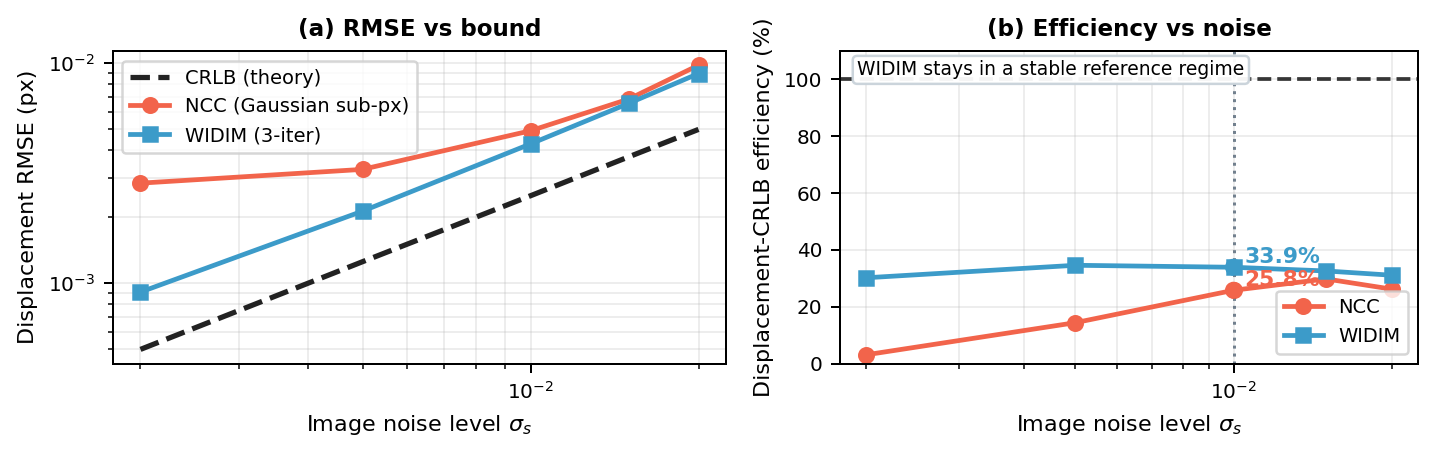
\includegraphics[width=0.82\textwidth]{figures/appendix/figA01_disp_crlb_reference.png}
  \caption{Reference displacement-path bound under pure translation
  ($u=4.37$\,px, $v=3.21$\,px, $WS=64$\,px, $N_{\mathrm{MC}}=200$).
  (a) Displacement RMSE versus image noise for the theoretical CRLB,
  NCC, and WIDIM. (b) Corresponding displacement-CRLB efficiency.
  This figure is included only to show that the WIDIM branch itself remains in a stable displacement regime.}
  \label{fig:app_disp_crlb}
\end{figure}

Fig.~\ref{fig:app_disp_crlb} is included only to show that the WIDIM
displacement branch itself remains in a stable displacement-reference-bound regime.
The flow-wise orthogonality check that is directly tied to the main argument
remains in the main paper, so that readers can verify the orthogonality between
the displacement and direct-rotation outputs while reading the method and the
primary experiments.

\section{Relationship Between No-Ground-Truth Proxy Metrics and True Improvement}
\label{app:proxy}

\subsection{Error Decomposition for Proxy RMSE/MAE Versus True RMSE}

Let the true local rotation-rate field be $\Omega$,
and let the WIDIM-gradient reference field be
\begin{equation}
  \Omega_{\mathrm{ref}} = \Omega + e_r,
  \label{eq:app_ref}
\end{equation}
where $e_r$ denotes the reference-field error.
For any estimator $m \in \{\mathrm{raw}, \mathrm{new}\}$ under comparison,
write
\begin{equation}
  \hat{\Omega}^{(m)} = \Omega + e_m.
  \label{eq:app_est}
\end{equation}

Then the proxy mean-squared error relative to the reference field is
\begin{align}
  \MSE_{\mathrm{proxy}}^{(m)}
  &= \E\!\left[\left(\hat{\Omega}^{(m)}-\Omega_{\mathrm{ref}}\right)^2\right] \nonumber\\
  &= \E\!\left[\left(e_m-e_r\right)^2\right] \nonumber\\
  &= \E[e_m^2] + \E[e_r^2] - 2\,\E[e_m e_r].
  \label{eq:app_proxy_mse}
\end{align}
whereas the true mean-squared error is
\begin{equation}
  \MSE_{\mathrm{true}}^{(m)} = \E[e_m^2].
  \label{eq:app_true_mse}
\end{equation}

Comparing the old and new estimators gives
\begin{align}
  \Delta \MSE_{\mathrm{proxy}}
  &\triangleq \MSE_{\mathrm{proxy}}^{(\mathrm{raw})}
    - \MSE_{\mathrm{proxy}}^{(\mathrm{new})} \nonumber\\
  &= \Delta \MSE_{\mathrm{true}}
  - 2\!\left(\E[e_{\mathrm{raw}}e_r]-\E[e_{\mathrm{new}}e_r]\right).
  \label{eq:app_delta_proxy}
\end{align}

Equation~\eqref{eq:app_delta_proxy} shows that when the reference-field error
$e_r$ is approximately fixed under the same gated mask,
and when the change in its correlation with the old and new estimators is small,
$\Delta \MSE_{\mathrm{proxy}}$ and $\Delta \MSE_{\mathrm{true}}$
tend to preserve the same sign.
Because the square root is monotone on the positive real line,
$\Delta \mathrm{RMSE}_g$ inherits the same improvement direction.
For approximately symmetric, near-zero-mean error distributions,
$\Delta \mathrm{MAE}_g$ also tends to align with the true RMSE gain,
although its monotonicity is weaker than the quadratic form behind
$\Delta \mathrm{RMSE}_g$.

For this reason, the main paper treats
$\Delta \mathrm{RMSE}_g$ and
$\Delta \mathrm{MAE}_g$
as the primary proxy metrics on real data without ground truth.
The logic is not that ``the reference field equals the truth'',
but that under a unified gated mask the reference-error term is shared to first
order by both estimators, so that the relative gain still maps to the direction
of true improvement.

\subsection{Why $\Delta \mathrm{Corr}_g$ Is Only Supporting Evidence}

The correlation coefficient is
\begin{equation}
  \mathrm{Corr}\!\left(\hat{\Omega},\Omega_{\mathrm{ref}}\right)
  = \frac{\Cov(\hat{\Omega},\Omega_{\mathrm{ref}})}
  {\sqrt{\Var(\hat{\Omega})\,\Var(\Omega_{\mathrm{ref}})}}.
  \label{eq:app_corr}
\end{equation}
Unlike RMSE, correlation is simultaneously affected by the covariance term,
variance normalization on both sides,
and the intrinsic dynamic range of the scene.
When the true flow variance is already small
(for example in pure solid rotation or near-linear shear),
the absolute error may decrease while correlation changes only weakly,
or even fails to track the true improvement monotonically.

On real data without ground truth,
$\Delta \mathrm{Corr}_g$ is therefore better interpreted as supporting evidence for
improved structural agreement or shape preservation.
It is weaker as a primary proxy metric than
$\Delta \mathrm{RMSE}_g$ or $\Delta \mathrm{MAE}_g$.

\subsection{Empirical Calibration on Synthetic Ground Truth}

The above analysis still requires empirical calibration on synthetic flows with
ground truth.
We therefore use a separate 20-seed calibration set and evaluate
80 flow-seed cases across Rankine, Lamb-Oseen, solid rotation, and linear shear.
For each case we compute
$\Delta \mathrm{Corr}_g$,
$\Delta \mathrm{RMSE}_g$,
$\Delta \mathrm{MAE}_g$,
and the corresponding
$\Delta \mathrm{RMSE}_{\mathrm{true}}$.

Table~\ref{tab:app_proxy} and Fig.~\ref{fig:app_proxy_scatter} jointly show that:
\begin{itemize}
  \item over all 80 cases, $\Delta \mathrm{RMSE}_g$ provides the most stable map to the true gain
  (Pearson $=0.994$, sign agreement $=86.2\%$);
  \item $\Delta \mathrm{MAE}_g$ is second strongest
  (Pearson $=0.977$, sign agreement $=88.8\%$);
  \item $\Delta \mathrm{Corr}_g$ still aligns with true improvement on average,
  but becomes visibly less stable in low-variance scenes and is therefore
  better treated as a supporting proxy only.
\end{itemize}
In the Rankine setting used for the primary experiment in the main paper,
all three proxy metrics reach a sign-agreement rate of $95\%$ with the true gain.
This is what allows the real-data section to be stated rigorously as a
calibrated proxy validation rather than an uncalibrated reference-field comparison.

\begin{table}[!t]
  \centering
  \caption{Proxy-to-truth calibration summary.
  Pearson and Spearman report linear and rank-order association between the
  proxy gain and $\Delta\mathrm{RMSE}_{\mathrm{true}}$;
  Sign reports directional agreement.}
  \label{tab:app_proxy}
  \scriptsize
  \renewcommand{\arraystretch}{1.10}
  \setlength{\tabcolsep}{4pt}
  \begin{tabular}{@{}llccc@{}}
    \toprule
    Metric & Flow type & Pearson & Spearman & Sign \\
    \midrule
    $\Delta \mathrm{Corr}_g$ & All synthetic ($N=80$) & 0.963 & 0.433 & 76.2\% \\
    $\Delta \mathrm{Corr}_g$ & Rankine ($N=20$) & 0.970 & 0.983 & 95.0\% \\
    $\Delta \mathrm{Corr}_g$ & Lamb-Oseen ($N=20$) & 1.000 & 0.562 & 75.0\% \\
    $\Delta \mathrm{Corr}_g$ & Solid rotation ($N=20$) & 0.054 & $-0.068$ & 65.0\% \\
    $\Delta \mathrm{Corr}_g$ & Linear shear ($N=20$) & $-0.150$ & $-0.084$ & 70.0\% \\
    \midrule
    $\Delta \mathrm{RMSE}_g$ & All synthetic ($N=80$) & 0.994 & 0.216 & 86.2\% \\
    $\Delta \mathrm{RMSE}_g$ & Rankine ($N=20$) & 0.999 & 0.986 & 95.0\% \\
    $\Delta \mathrm{RMSE}_g$ & Lamb-Oseen ($N=20$) & 1.000 & 0.173 & 75.0\% \\
    $\Delta \mathrm{RMSE}_g$ & Solid rotation ($N=20$) & 0.389 & 0.203 & 90.0\% \\
    $\Delta \mathrm{RMSE}_g$ & Linear shear ($N=20$) & 0.433 & 0.541 & 85.0\% \\
    \midrule
    $\Delta \mathrm{MAE}_g$ & All synthetic ($N=80$) & 0.977 & 0.238 & 88.8\% \\
    $\Delta \mathrm{MAE}_g$ & Rankine ($N=20$) & 0.962 & 0.965 & 95.0\% \\
    $\Delta \mathrm{MAE}_g$ & Lamb-Oseen ($N=20$) & 0.995 & 0.311 & 75.0\% \\
    $\Delta \mathrm{MAE}_g$ & Solid rotation ($N=20$) & 0.494 & 0.188 & 100.0\% \\
    $\Delta \mathrm{MAE}_g$ & Linear shear ($N=20$) & 0.510 & 0.541 & 85.0\% \\
    \bottomrule
  \end{tabular}
\end{table}

\begin{figure}[!t]
  \centering
  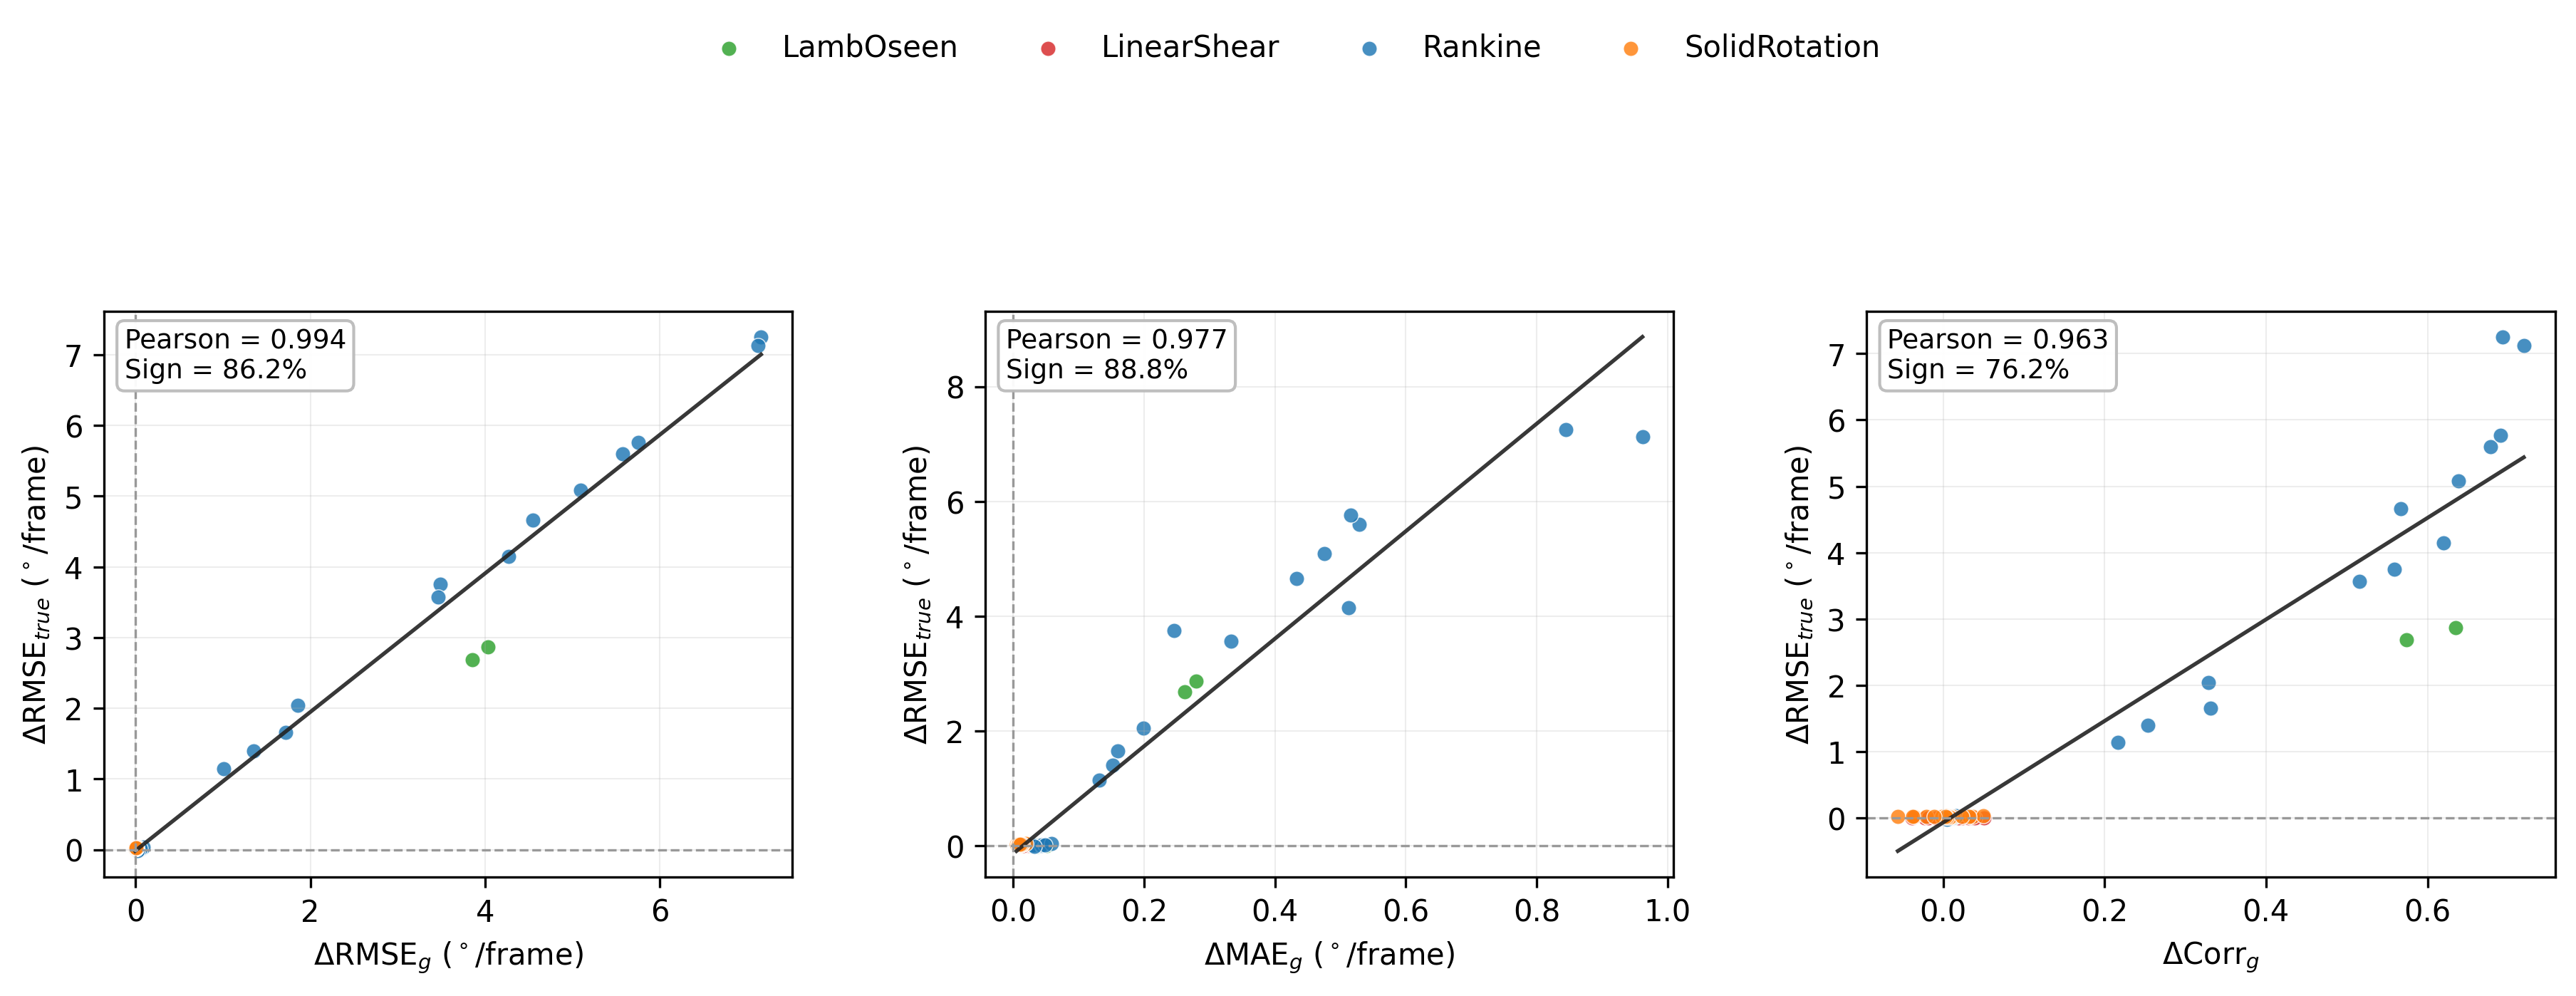
\includegraphics[width=\textwidth]{figures/appendix/figA02_proxy_calibration.png}
  \caption{Empirical calibration of real-data proxy gains against ground-truth RMSE gain
  on the separate 20-seed synthetic calibration set.
  The left and middle panels show that
  $\Delta \mathrm{RMSE}_g$ and $\Delta \mathrm{MAE}_g$
  remain strongly aligned with
  $\Delta \mathrm{RMSE}_{\mathrm{true}}$.
  The right panel shows that
  $\Delta \mathrm{Corr}_g$ is still positively associated overall,
  but is more scene-dependent and therefore used only as supporting evidence.}
  \label{fig:app_proxy_scatter}
\end{figure}

To make the calibration easier to assess flow by flow,
Fig.~\ref{fig:app_proxy_by_flow} isolates the primary proxy
$\Delta \mathrm{RMSE}_g$ within each synthetic flow.
The Rankine and Lamb--Oseen panels retain very strong directional consistency,
whereas solid rotation and linear shear are visibly weaker because their
intrinsic rotation-rate dynamic range is much smaller.
This is exactly why the main paper treats the real-data proxy as a calibrated
deployment-side indicator rather than as a direct replacement for ground truth.

\begin{figure}[!t]
  \centering
  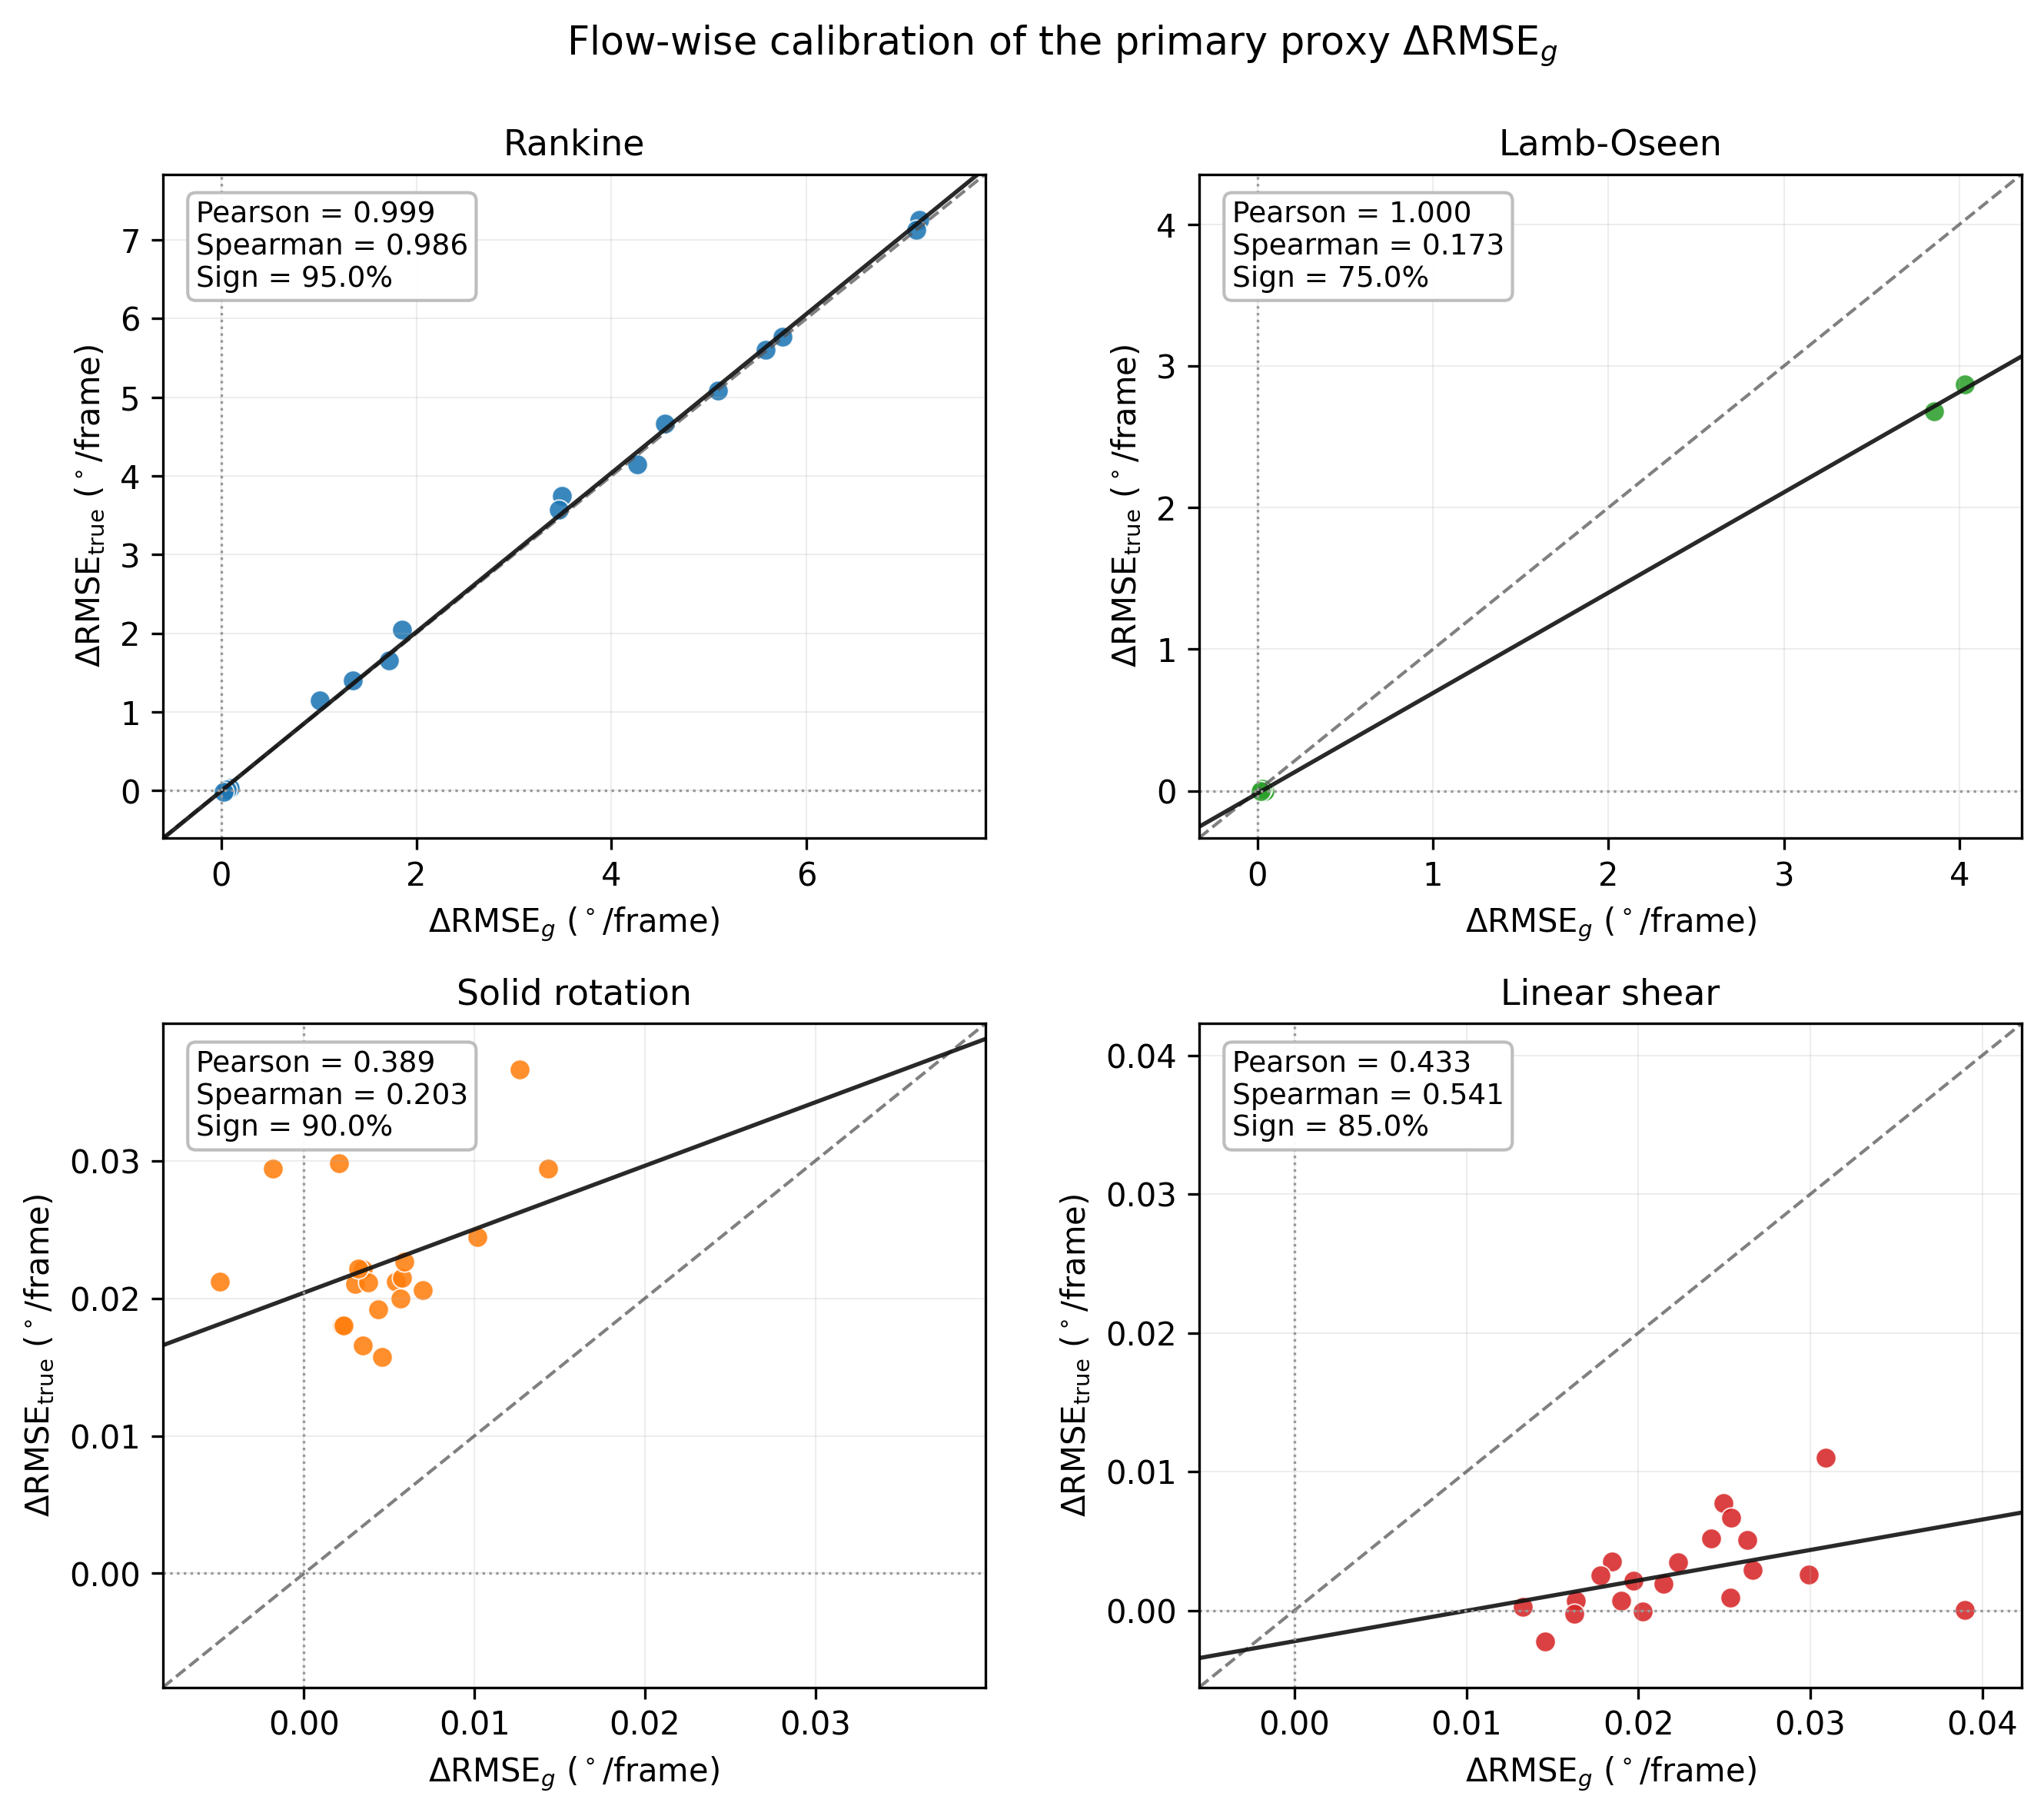
\includegraphics[width=0.92\textwidth]{figures/appendix/figA03_proxy_by_flow.png}
  \caption{Flow-wise calibration of the primary proxy $\Delta \mathrm{RMSE}_g$.
  Each panel compares the proxy gain to the true RMSE gain on one synthetic flow.
  The dashed diagonal indicates perfect magnitude agreement.
  Across flows, the directional agreement remains strongest in Rankine and
  remains acceptable in the lower-variance solid-rotation and linear-shear settings.}
  \label{fig:app_proxy_by_flow}
\end{figure}

Fig.~\ref{fig:app_proxy_rankine} further focuses on the Rankine setting used by
the primary experiment in the main text.
In this matched scenario, all three proxy metrics reach a $95\%$ sign-agreement
rate with the true gain, which is the most relevant calibration fact supporting
the real-data discussion in the manuscript.

\begin{figure}[!t]
  \centering
  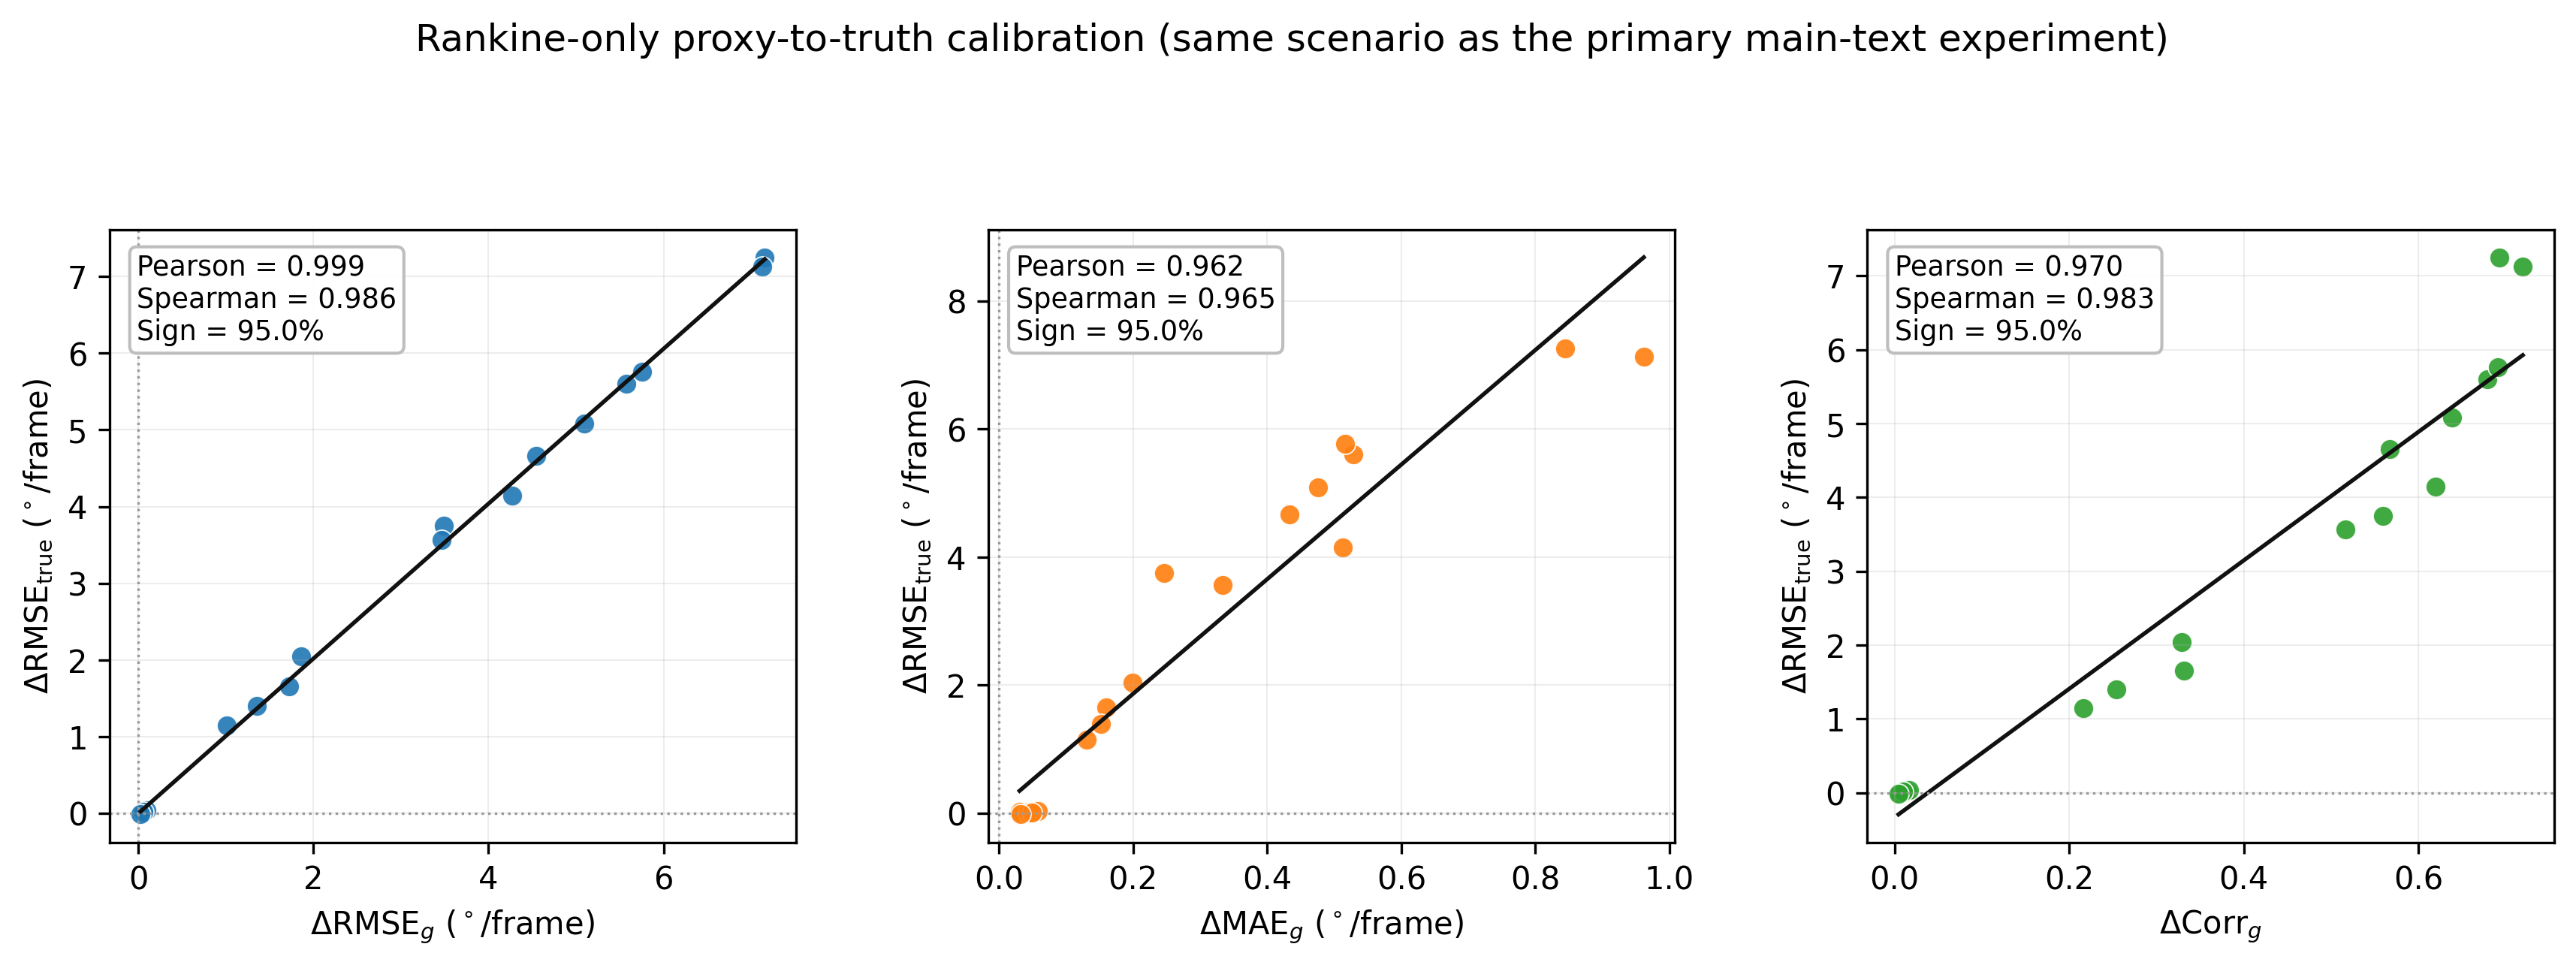
\includegraphics[width=\textwidth]{figures/appendix/figA04_rankine_proxy_triplet.png}
  \caption{Rankine-only proxy-to-truth calibration on the same class of synthetic
  scenario used by the primary main-text experiment.
  In this matched setting,
  $\Delta \mathrm{RMSE}_g$, $\Delta \mathrm{MAE}_g$, and $\Delta \mathrm{Corr}_g$
  all remain strongly aligned in sign with
  $\Delta \mathrm{RMSE}_{\mathrm{true}}$,
  while the error-based proxies remain the most stable in magnitude.}
  \label{fig:app_proxy_rankine}
\end{figure}

\FloatBarrier
\section{Additional Rationale for Deployment-Side Design Choices}
\label{app:deploy}

\subsection{Why Translation-Only Alignment Is Used Instead of Affine De-rotation}

Within a local window, a small-deformation motion can be written as
\begin{equation}
  \mathbf{x}' = \mathbf{x} + \mathbf{t} + \mathbf{J}\mathbf{x},
  \qquad
  \mathbf{J} = \mathbf{S} + \mathbf{A},
  \label{eq:app_affine}
\end{equation}
where $\mathbf{t}$ is the translation term,
$\mathbf{S}$ is the symmetric deformation component,
and $\mathbf{A}$ is the antisymmetric component.
In two dimensions,
\begin{equation}
  \mathbf{A} =
  \begin{bmatrix}
    0 & -\Omega \\
    \Omega & 0
  \end{bmatrix},
  \label{eq:app_antisym}
\end{equation}
which is exactly the local rotation-rate signal that the paper seeks to estimate
directly through spectral angular shift.

If a full affine inverse transform containing the antisymmetric component is
applied before NUFFT estimation,
it removes not only translational mismatch but also part of the target
rotational signal itself.
The residual window faced by the direct estimator would then no longer match the
theoretical measurement object defined in the main text.
By contrast, translation-only alignment removes the gross window-center mismatch
while preserving the local rotational component for NUFFT estimation.
This is why the final deployable protocol insists that
``WIDIM is used only for window tracking and translation prior''
rather than for affine de-rotation.

\begin{figure}[!t]
  \centering
  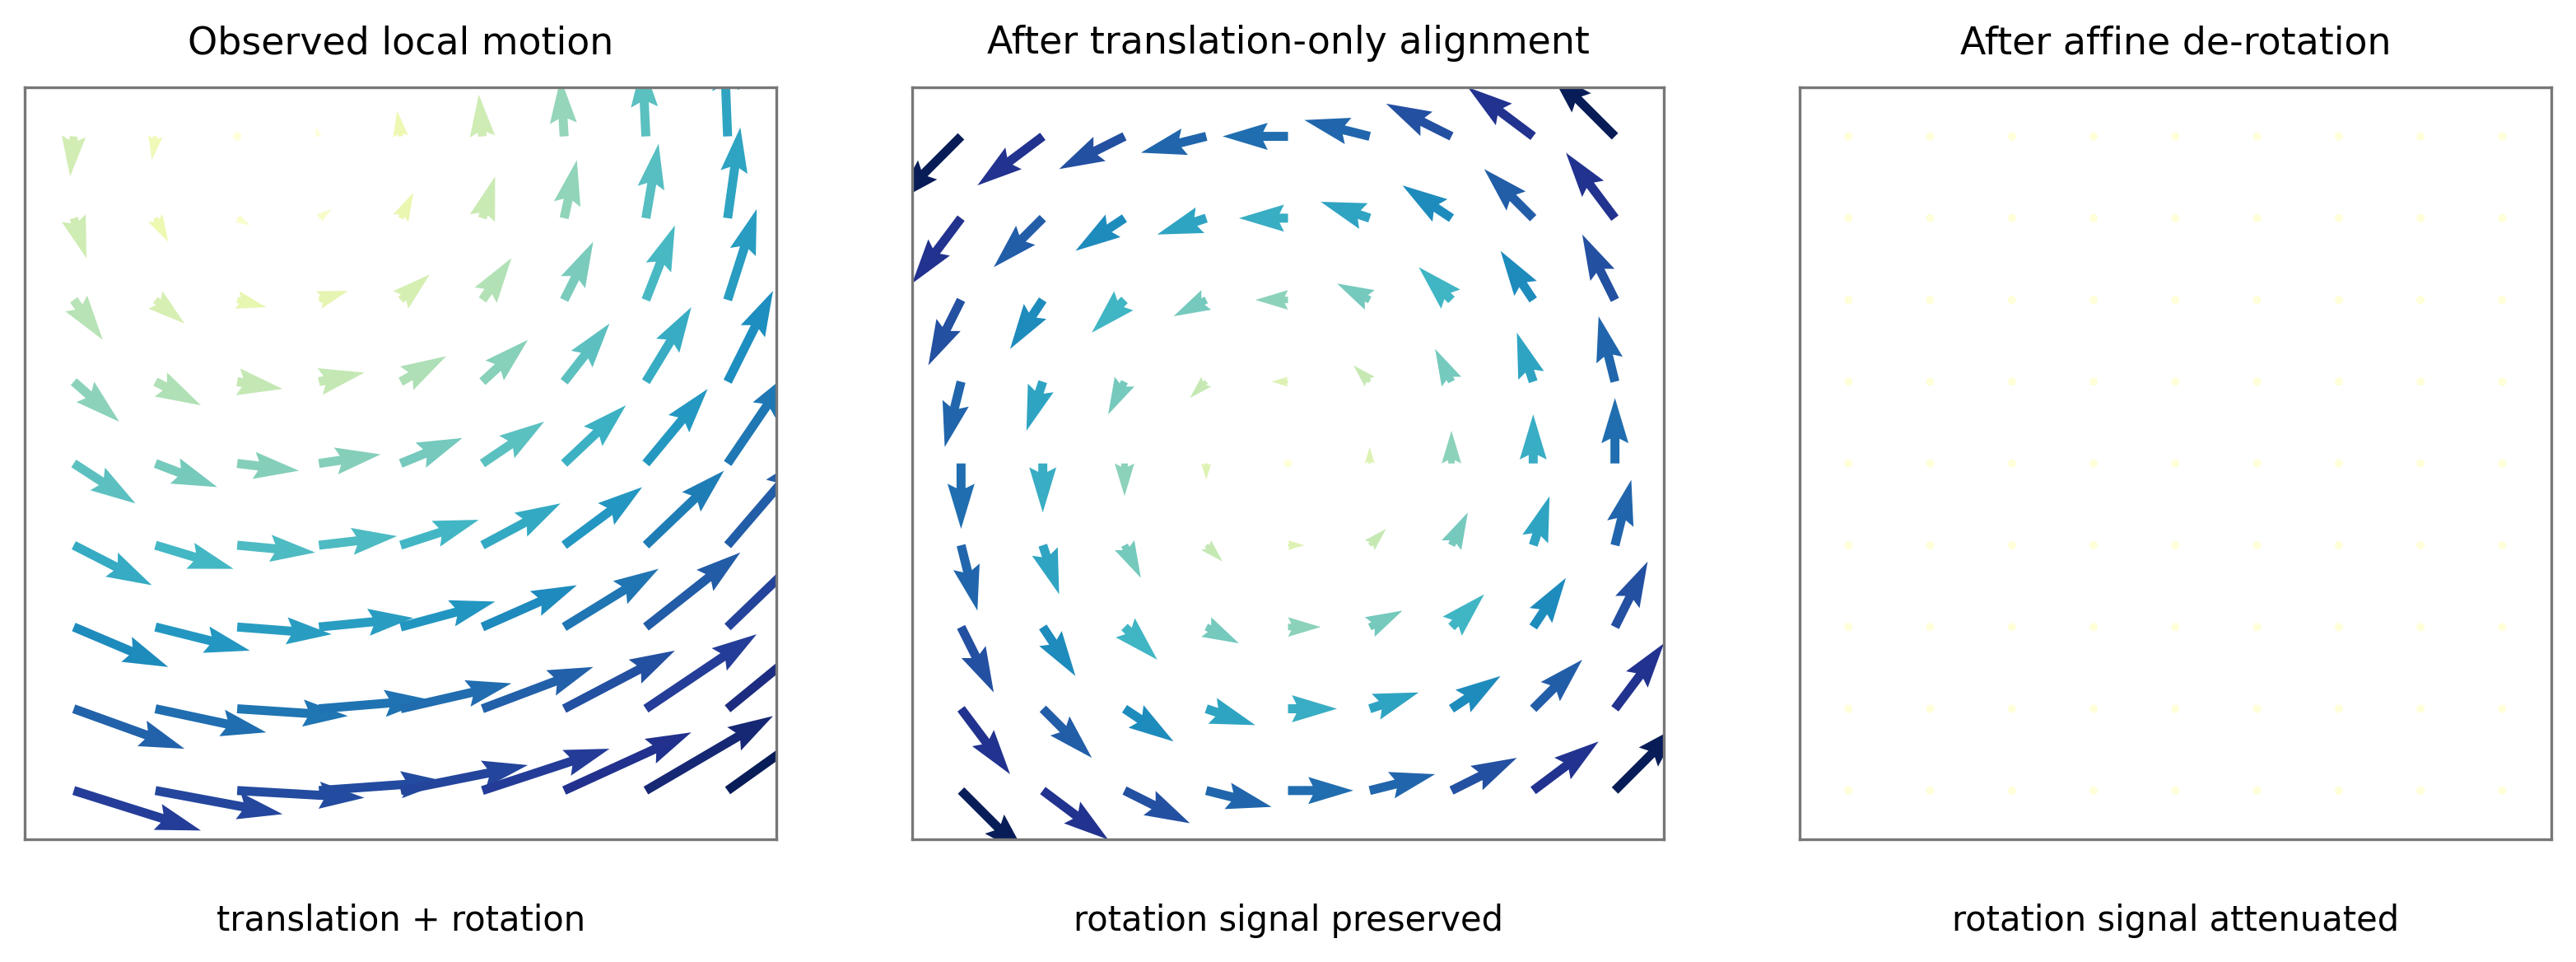
\includegraphics[width=\textwidth]{figures/appendix/figA05_translation_vs_affine.png}
  \caption{Why the deployable protocol uses translation-only alignment before NUFFT.
  Left: observed local motion contains both translation and rotation.
  Middle: translation-only alignment removes the gross displacement mismatch but preserves the rotational component.
  Right: affine de-rotation suppresses the antisymmetric component itself, thereby attenuating the target signal to be estimated.}
  \label{fig:app_affine}
\end{figure}

\subsection{Why Adaptive p5 Gating Is Used Instead of a Fixed SNR Threshold}

The quality distribution of local windows on real data varies substantially with
the source pool, imaging conditions, and particle density.
An absolute SNR threshold therefore does not carry a uniform meaning across pairs.
In the executed 320-pair batch, the pair-wise p5 threshold spans
$1.299$--$2.743$ globally.
Grouped by source, the mean thresholds are
$2.161$ for PIV-C,
$1.474$ for PIV-E,
and $1.815$ for PIV-book.
If a single fixed threshold such as 2.2 is used,
it sits near the lower-tail threshold of PIV-C but well above the typical
threshold of PIV-E,
which means that it implies fundamentally different rejection rates in
different source pools.

This would destroy a unified evaluation policy across datasets:
the observed performance change would become entangled with how many windows were
retained, rather than reflecting only the estimator and the post-processing logic.
By contrast, the adaptive p5 gate rejects the lowest-confidence 5\% of windows
on each image pair.
The gate is therefore interpreted as a fixed tail-rejection policy rather than
as a one-size-fits-all threshold on the absolute SNR value.

\begin{figure}[!t]
  \centering
  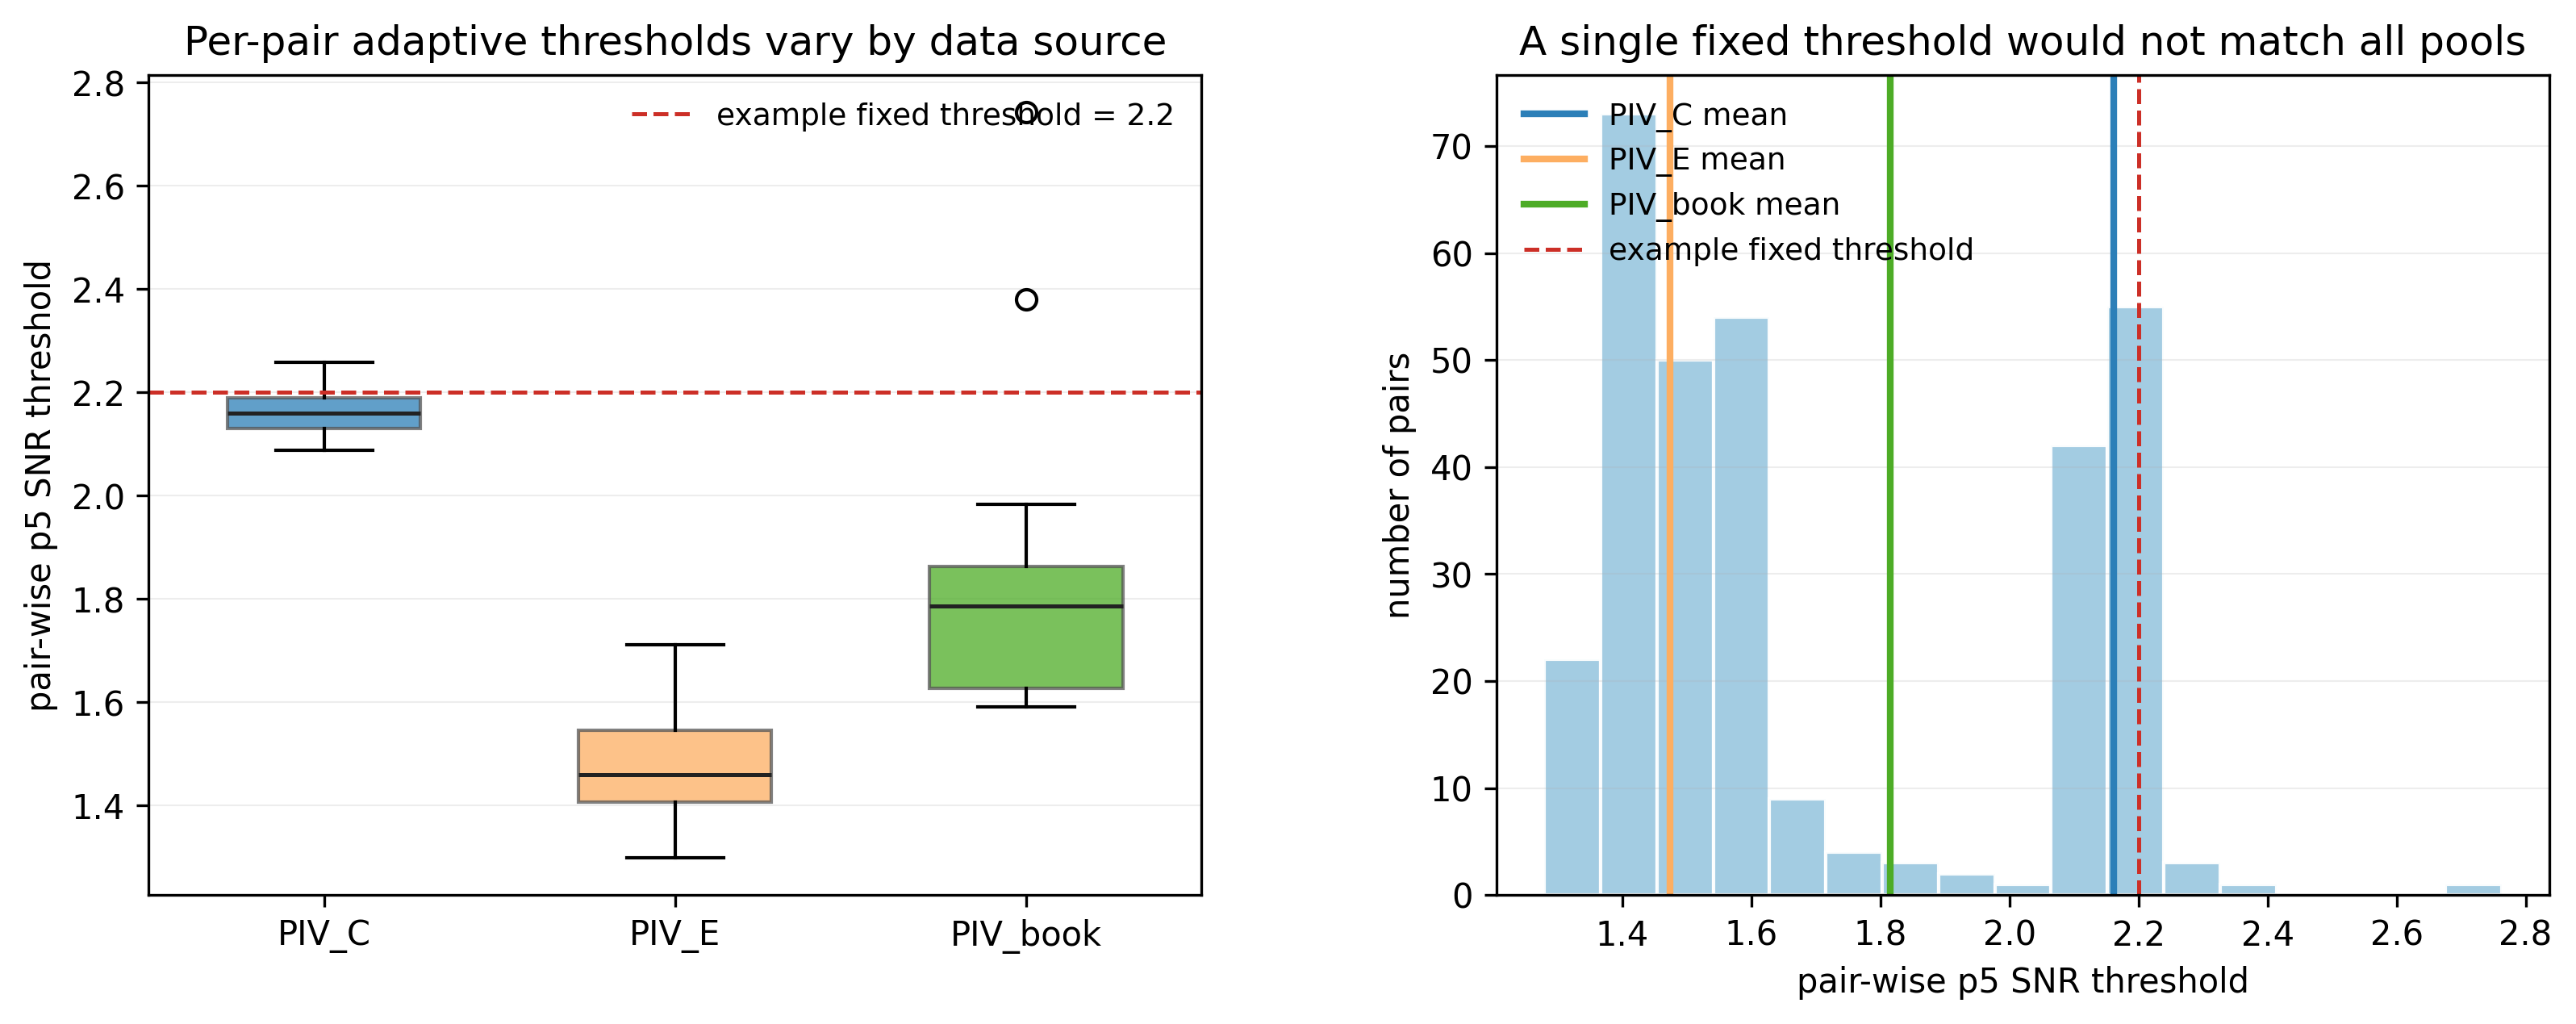
\includegraphics[width=\textwidth]{figures/appendix/figA06_gate_percentile.png}
  \caption{Why a percentile gate is preferable to a single fixed SNR threshold on real data.
  Left: pair-wise p5 thresholds vary substantially across sources.
  Right: the threshold distribution shows that one fixed cutoff would correspond to different effective rejection policies on different data pools.
  The percentile gate instead keeps the tail-rejection rule fixed across pairs.}
  \label{fig:app_gate}
\end{figure}

\subsection{Held-Out Subset Audit: No Gate Versus Adaptive p5}

Fig.~\ref{fig:app_gate_audit} reports a small held-out audit on the 11 PIV-book cam1 pairs
for which both a no-gate result and an adaptive-p5 result are available under the same
track-prior NUFFT pipeline.
It provides an additional deployment-side check on the effect of adaptive p5 gating.

On this subset, the adaptive p5 version improves the proxy RMSE on all 11 pairs
($5.527 \rightarrow 2.566$ on average) and the proxy MAE on all 11 pairs
($2.616 \rightarrow 1.427$ on average),
while also improving the proxy correlation on 8 of the 11 pairs
($0.0779 \rightarrow 0.1106$ on average).
Combined with Fig.~\ref{fig:app_gate},
this audit supports the interpretation that p5 is not an arbitrary tuning knob:
the percentile rule provides a source-independent tail-rejection policy,
and the resulting gain remains observable when compared against the no-gate version
on a held-out real subset.

\begin{figure}[!t]
  \centering
  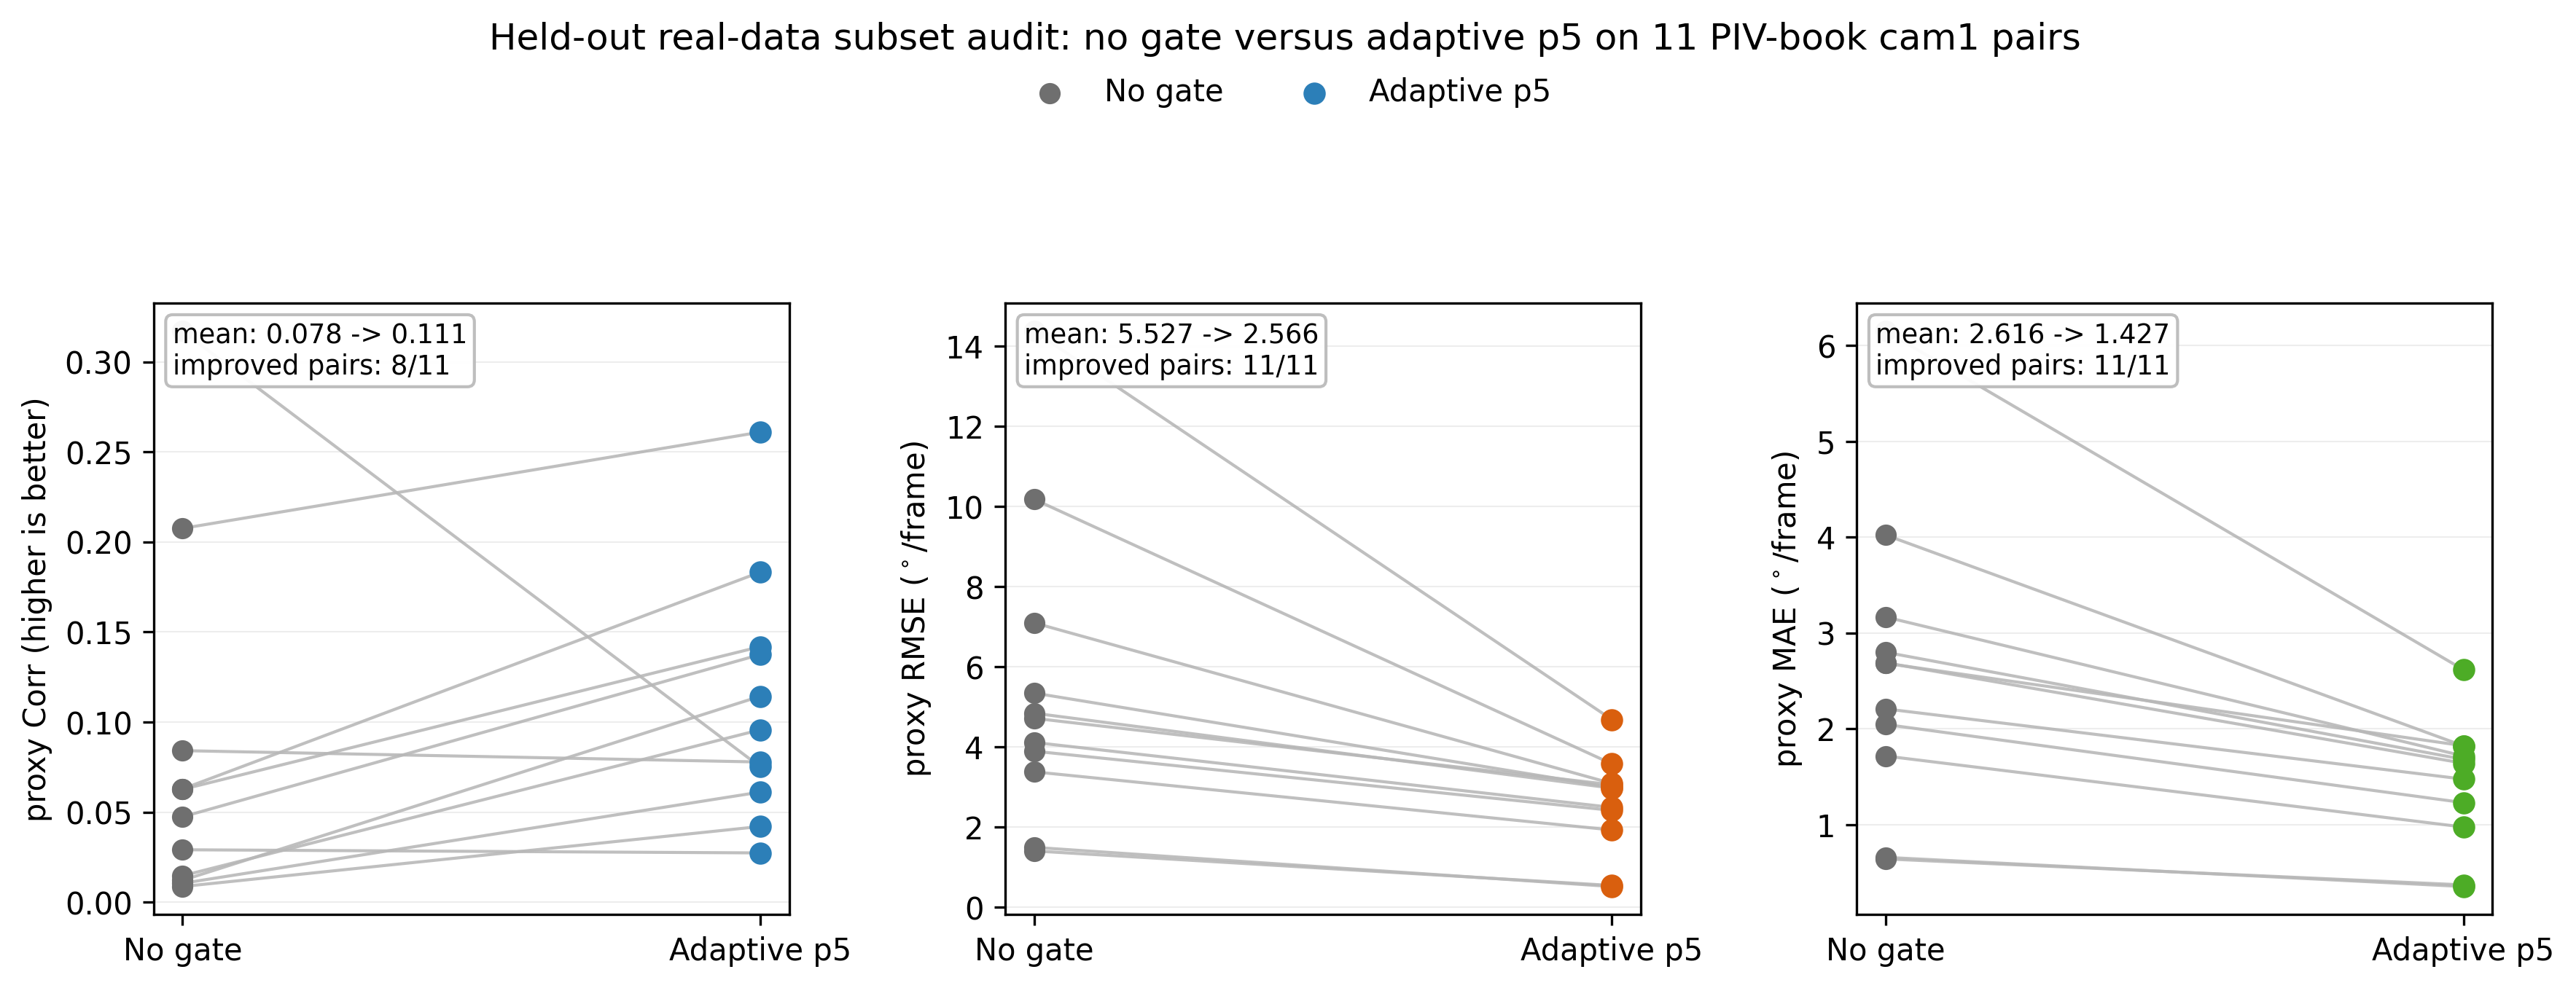
\includegraphics[width=\textwidth]{figures/appendix/figA07_gate_subset.png}
  \caption{Held-out audit of no gate versus adaptive p5 on 11 PIV-book cam1 pairs.
  Each line joins the same image pair under the two gating policies.
  Adaptive p5 improves the proxy RMSE and proxy MAE on all 11 pairs,
  and improves the proxy correlation on 8 of the 11 pairs.
  This figure provides a minimal robustness check that the real-data conclusion is
  not created only by one accidental gate choice.}
  \label{fig:app_gate_audit}
\end{figure}

\subsection{Finite-Window Particle Loss and Tail-Variance Suppression}

The main text now discusses the deployment-side mechanism at the level of
physical interpretation only.
This subsection records the minimal supporting model that connects finite-window
particle loss, low-SNR mismatches, and the observed reduction of long-tail proxy
errors.

In a finite Eulerian window of side length $N$, a frame-to-frame displacement
magnitude $|d|$ causes a first-order particle-loss fraction of
\begin{equation}
  F_{\rm loss} \approx \frac{|d|}{N},
  \label{eq:app_particle_loss}
\end{equation}
which is the same scaling used in the main-text controlled protocol analysis.
When $N=64$\,px and $|d|=10$\,px, the implied loss is already on the order of
15\%.
This breaks the exact infinite-domain shift-invariance premise of the spectral
measurement object, broadens the polar cross-correlation peak, and lowers the
local SNR.

To express the statistical consequence in the smallest possible form, write the
local rotation-angle estimate as
\begin{equation}
  \hat{\alpha} = \alpha + b + \varepsilon,
  \qquad
  \E[\varepsilon]=0,\ \Var(\varepsilon)=\sigma_\varepsilon^2,
  \label{eq:app_minerr}
\end{equation}
where $b$ absorbs systematic bias from finite-window truncation or local
misregistration, and $\varepsilon$ represents the random component.
If $G\in\{0,1\}$ denotes the combined validity mask after two-pass spatial
post-processing and adaptive p5 gating, then the gated mean-squared error
becomes
\begin{equation}
  \E\!\left[(\hat{\alpha}-\alpha)^2 \mid G=1\right]
  = b_G^2 + \sigma_{\varepsilon,G}^2.
  \label{eq:app_gated_mse}
\end{equation}
The role of the gate is not to redefine the measurement object, but to reduce
the variance contribution of low-confidence windows, i.e., to move from
$\sigma_\varepsilon^2$ to a smaller $\sigma_{\varepsilon,G}^2$ under a fixed
tail-rejection policy.

The second-pass refill is likewise kept deliberately bounded.
If a rejected outlier $x_{ij}$ is replaced by a neighborhood statistic
$\phi(\mathcal{N}_{ij})$, then the implementation enforces
\begin{equation}
  \min\nolimits_{(p,q)\in\mathcal{N}_{ij}} x_{pq}
  \le \phi(\mathcal{N}_{ij})
  \le \max\nolimits_{(p,q)\in\mathcal{N}_{ij}} x_{pq},
  \label{eq:app_bounded_refill}
\end{equation}
so that the refill cannot introduce an unbounded excursion beyond the local
range already supported by neighboring windows.

This supporting derivation clarifies the qualitative main-text claim:
on difficult real images, the final protocol often improves first by suppressing
variance-heavy catastrophic windows; on vortex-dominated scenes with stronger
coherent organization, the same protocol can additionally reveal a clearer
structural gain.

\FloatBarrier
\section{Additional Theoretical Diagnostics}
\label{app:theory_extra}

\subsection{Radial SNR Profile and the High-SNR Assumption}

The CRLB analysis in the main text assumes that the dominant angular-information bins
still operate in a usable high-SNR regime.
Fig.~\ref{fig:app_a3} therefore reports the radial amplitude profile,
the corresponding $\mathrm{SNR}_{\mathrm{amp}}(r)$ curves,
and the Fisher-information distribution under unweighted and $r^2$ weighting.
The figure is included to show which part of the polar spectrum actually carries
most of the usable angular information, and why the Gaussian-noise approximation
should be interpreted as an operating-range assumption rather than a claim about
all radial bins.

\begin{figure}[!t]
  \centering
  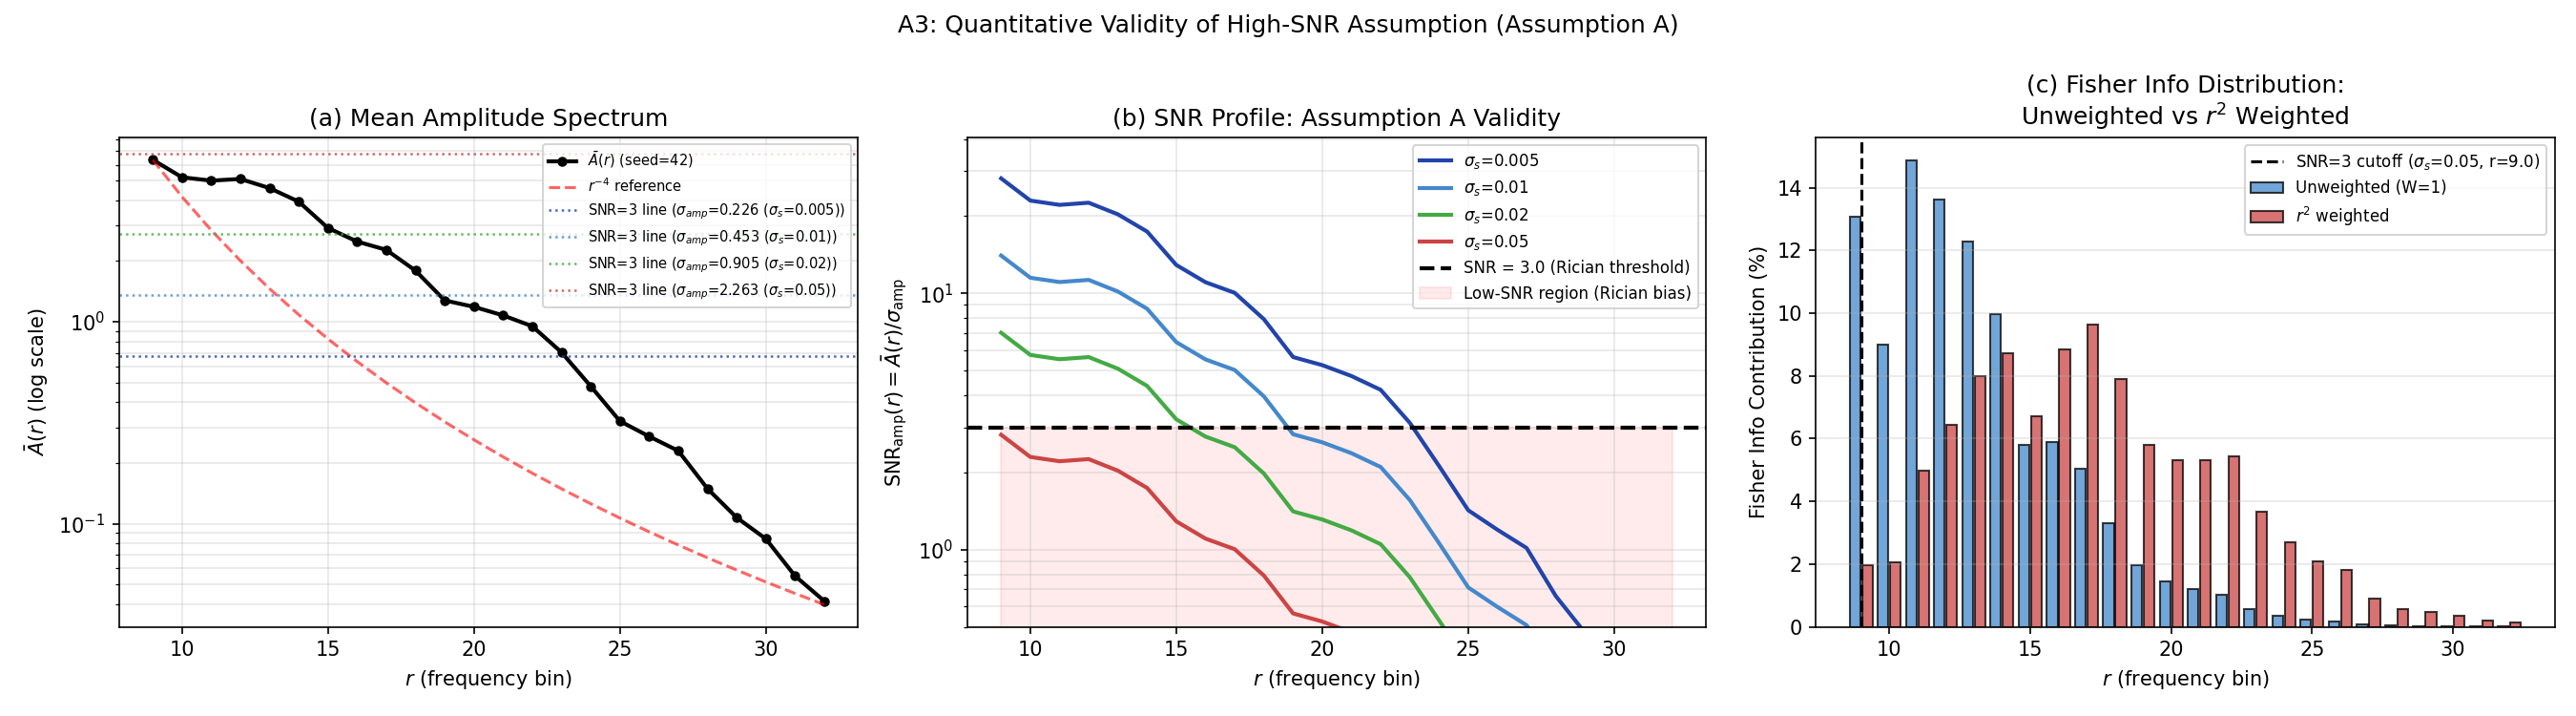
\includegraphics[width=\textwidth]{figures/appendix/figA08_snr_profile.png}
  \caption{A3 diagnostic for the high-SNR assumption.
  (a) Radial mean amplitude spectrum.
  (b) Radial amplitude-SNR profile for multiple image-noise levels.
  (c) Fisher-information distribution with and without $r^2$ weighting.
  The figure clarifies where the usable angular information is concentrated and
  why the high-SNR approximation is expected to hold only over a restricted operating range.}
  \label{fig:app_a3}
\end{figure}

\subsection{Multi-seed Stability of the CRLB Hierarchy}

To rule out the possibility that the CRLB hierarchy is an artifact of one random
speckle realization, Fig.~\ref{fig:app_b3} repeats the calculation across 10 independent seeds.
Although the absolute Fisher information changes with the texture realization,
the hierarchy ordering and the retained-information ratio after radial integration remain stable.
This supports the interpretation that the hierarchy reported in the main text is
a property of the measurement path rather than a single fortunate sample.

\begin{figure}[!t]
  \centering
  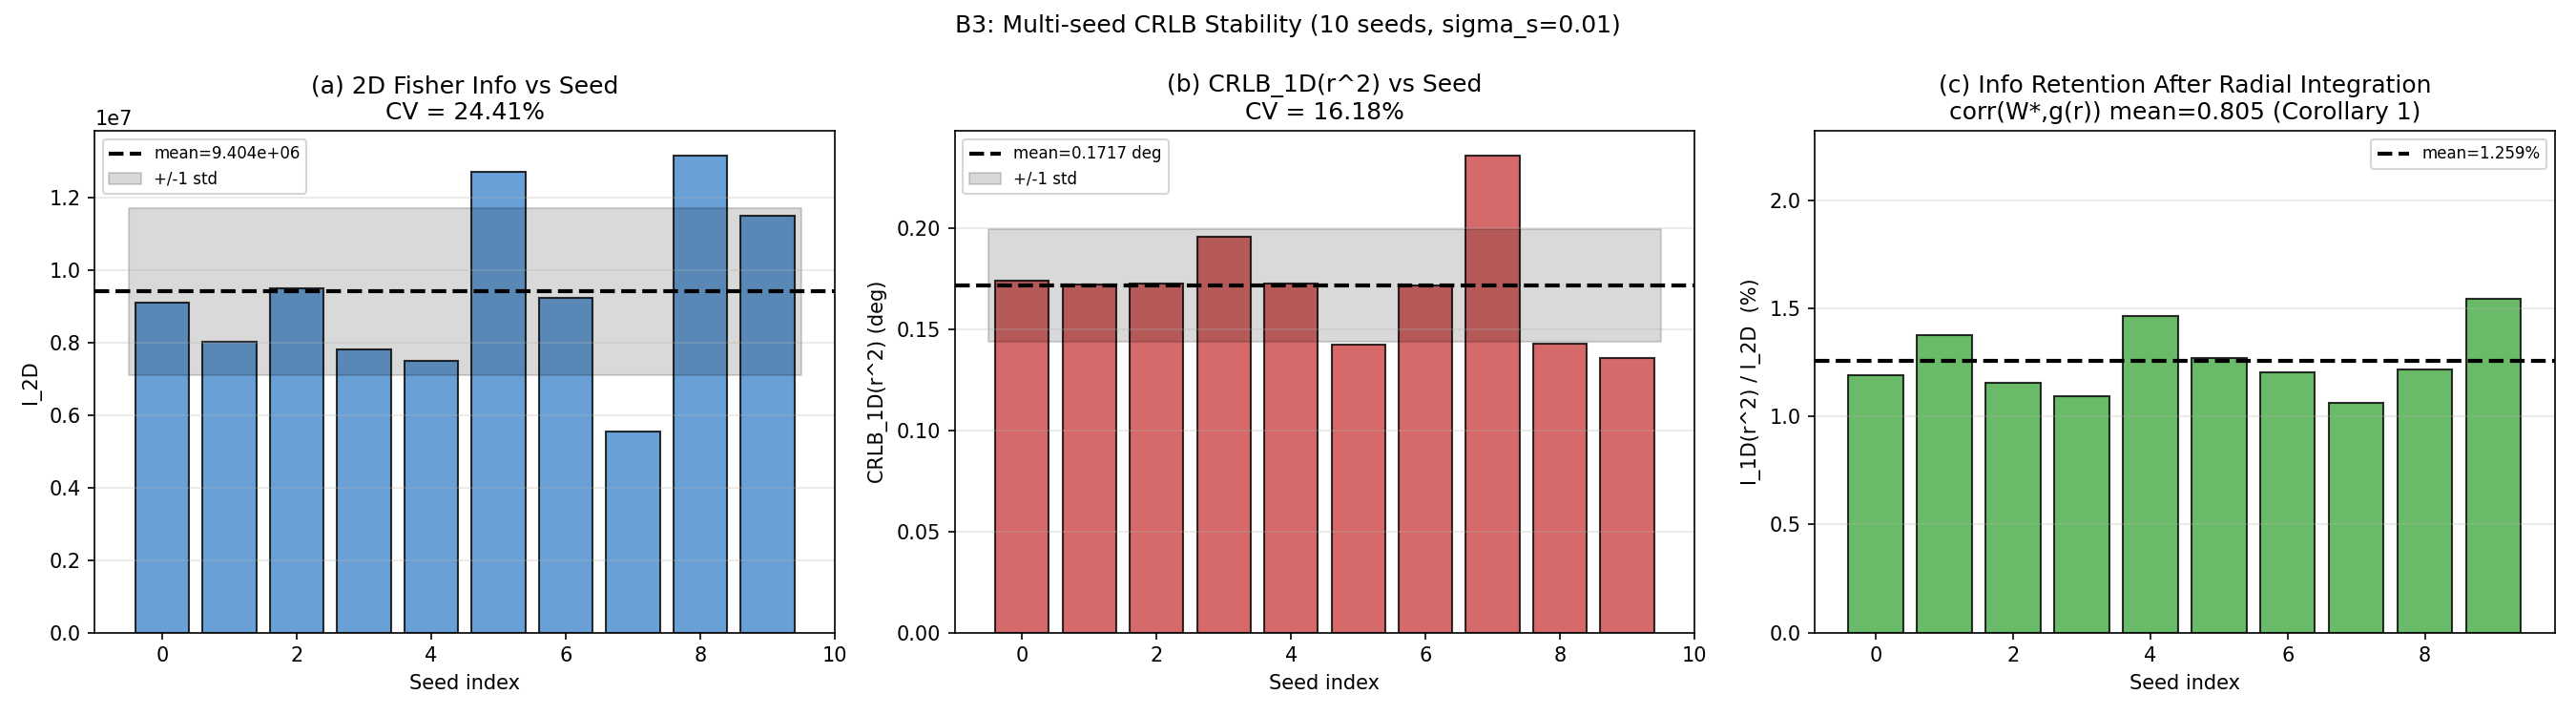
\includegraphics[width=\textwidth]{figures/appendix/figA09_multiseed_stability.png}
  \caption{B3 diagnostic for multi-seed stability of the CRLB hierarchy.
  The three panels report cross-seed variation of the 2D Fisher information,
  the resulting $\mathrm{CRLB}_{1D}(r^2)$, and the retained-information ratio
  $I_{1D}(r^2)/I_{2D}$.
  The hierarchy remains stable across seeds even though the absolute values fluctuate with the random speckle pattern.}
  \label{fig:app_b3}
\end{figure}

\subsection{Two-image Noise Model Validation}

The main-text CRLB calculations adopt the effective two-image noise model
$\sigma_{\mathrm{eff}}=\sqrt{2}\,\sigma_s$.
Fig.~\ref{fig:app_b4} validates this approximation numerically by comparing the
resulting theoretical bound with Monte Carlo RMSE under independently corrupted
image pairs.
The agreement is good over the practical operating range and breaks down only in
the extreme high-noise regime, where the estimator itself has already left the
usable operating region.

\begin{figure}[!t]
  \centering
  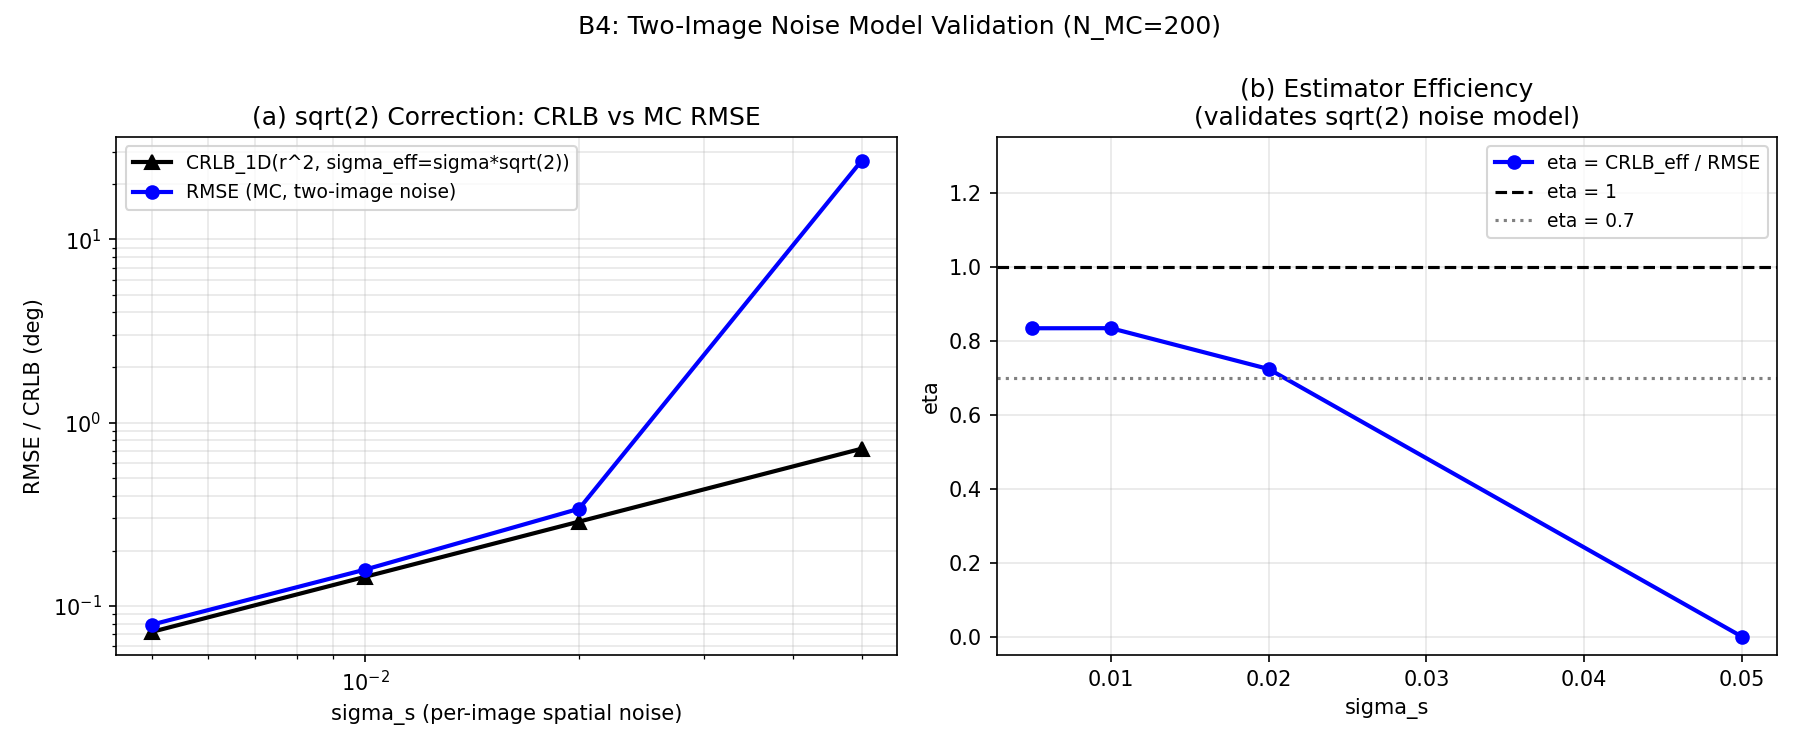
\includegraphics[width=\textwidth]{figures/appendix/figA10_noise_model_validation.png}
  \caption{B4 diagnostic for the effective two-image noise model.
  (a) Theoretical $\mathrm{CRLB}_{1D}$ obtained with
  $\sigma_{\mathrm{eff}}=\sqrt{2}\,\sigma_s$ versus Monte Carlo RMSE.
  (b) Corresponding estimator efficiency across noise levels.
  The approximation is accurate over the practical operating range and deviates only in the extreme high-noise regime.}
  \label{fig:app_b4}
\end{figure}

\subsection{Practical Efficiency-Gap Decomposition}

The main text keeps only the CRLB hierarchy figure and the final Rankine evidence.
The extra efficiency-gap decomposition is moved here because it is a supporting
diagnostic rather than a primary validation figure. Its role is to explain why a
direct estimator that approaches the ideal 1D bound under uniform rotation still
shows a larger gap once it is deployed at a practical Eulerian PIV operating point
with finite step size and finite angular resolution.

\begin{figure}[!t]
  \centering
  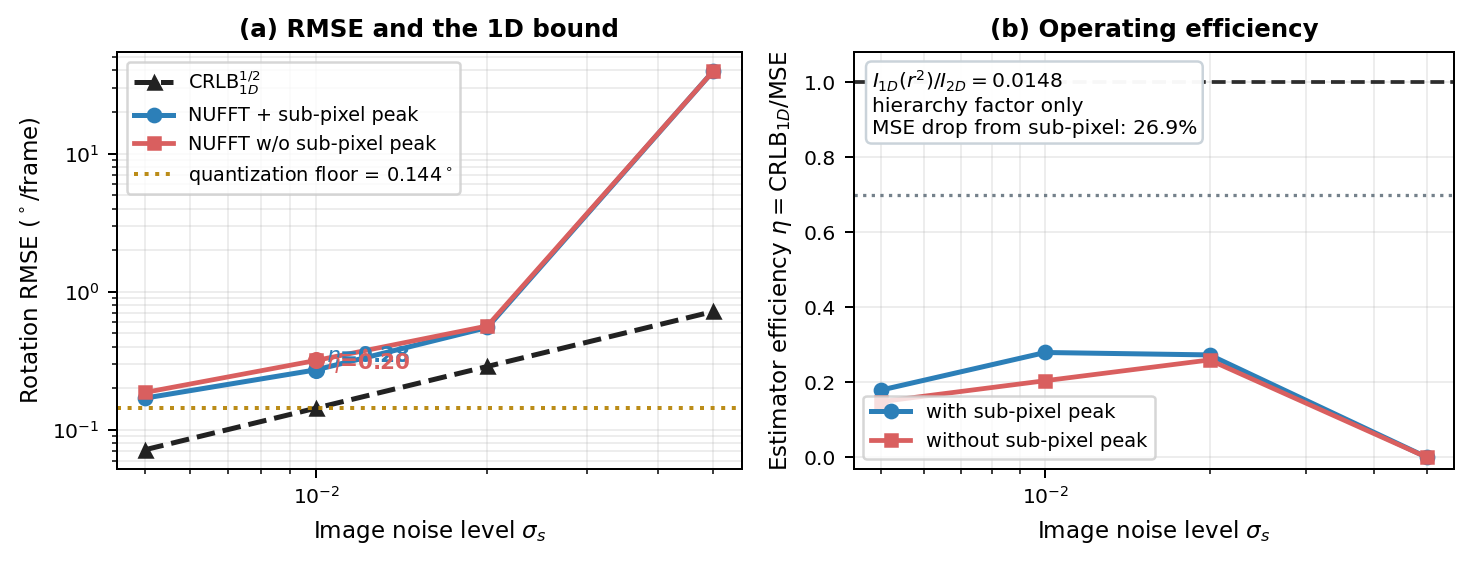
\includegraphics[width=\textwidth]{figures/appendix/fig05_efficiency_gap.png}
  \caption{Practical efficiency-gap decomposition between the ideal 1D bound and a representative
  Eulerian PIV operating point ($dx=10.0\,$px, $dy=7.8\,$px).
  (a) $\mathrm{CRLB}_{1D}^{1/2}$ and measured RMSE with and without sub-pixel peak fitting.
  (b) Corresponding estimator efficiency
  $\eta=\mathrm{CRLB}_{1D}/\mathrm{MSE}$.
  At $\sigma_s=0.01$, sub-pixel peak fitting raises $\eta$ from $0.204$ to $0.279$,
  indicating that part of the practical gap comes from peak localization rather than
  from the 1D-vs-2D hierarchy itself.}
  \label{fig:app_efficiency_gap}
\end{figure}

\FloatBarrier
\section{Dataset Organization and Additional Real-Data Summary}
\label{app:data}

This supplement also records the executed real-data organization used by the paper.
The full provenance spans five public origins, whereas the batch actually executed
for the real-data study is organized into three local pools totaling 320 image pairs.
Table~\ref{tab:app_sources} separates provenance from executable local organization,
which is helpful because the two single-pair challenge cases are kept only as provenance
records rather than standalone local folders in the current batch layout.

\begin{table}[!t]
  \centering
  \caption{Real-data provenance and executed local organization.}
  \label{tab:app_sources}
  \small
  \renewcommand{\arraystretch}{1.12}
  \setlength{\tabcolsep}{4pt}
  \begin{tabular}{@{}p{3.2cm}p{3.2cm}p{1.4cm}p{6.6cm}@{}}
    \toprule
    Origin & Current local organization & Executed pairs & Note \\
    \midrule
    PIV Challenge 2001 Case A & merged provenance entry & -- & Strong real-vortex single pair. Documented in the source map but not retained as a standalone local folder in the executed batch. \\
    PIV Challenge 2005 Case C & PIV\_C & 100 & Real jet / vortex-containing pool used directly in the 320-pair batch. \\
    PIV Challenge 2014 Case E & PIV\_E & 198 & Real vortex-ring sequence used directly in the 320-pair batch. \\
    PIV Challenge 2014 Case F & merged provenance entry & -- & Solid-body-rotation single pair. Documented for provenance but not retained as a standalone local folder in the executed batch. \\
    PIVbook stereo vortex ring & PIV\_book & 22 & Two-camera vortex-ring sample (cam1: 11 pairs, cam2: 11 pairs). \\
    \bottomrule
  \end{tabular}
\end{table}

Table~\ref{tab:app_real_sources} and Fig.~\ref{fig:app_real_sources}
summarize the executed real-data batch at the source level.
The table keeps the raw source-wise proxy gains in the supplement so that the main text
does not need to carry all dataset bookkeeping details, while the figure gives a quick
visual comparison across the three data pools.

\begin{table}[!t]
  \centering
  \caption{Source-wise summary of the executed 320-pair real-data batch.
  Positive $\Delta \mathrm{Corr}_g$ reports the percentage of pairs with improved structural agreement;
  $\Delta \mathrm{RMSE}_g$ is positive for every executed pair in all three pools.}
  \label{tab:app_real_sources}
  \small
  \renewcommand{\arraystretch}{1.12}
  \setlength{\tabcolsep}{4pt}
  \resizebox{\textwidth}{!}{%
  \begin{tabular}{@{}lrrrrrrrr@{}}
    \toprule
    Source pool & Pairs & Mean $\Delta \mathrm{RMSE}_g$ & Mean $\Delta \mathrm{MAE}_g$ & Mean $\Delta \mathrm{Corr}_g$ & Positive $\Delta \mathrm{Corr}_g$ & Mean p5 threshold & Mean pass rate & Mean time (s) \\
    \midrule
    PIV\_C    & 100 & 6.225 & 2.764 & 0.0057 & 62.0\% & 2.161 & 95.0\% & 298.6 \\
    PIV\_E    & 198 & 9.909 & 10.146 & 0.0032 & 51.0\% & 1.474 & 94.3\% & 282.8 \\
    PIV\_book & 22  & 5.101 & 3.915 & 0.0433 & 86.4\% & 1.815 & 95.1\% & 310.0 \\
    \bottomrule
  \end{tabular}}
\end{table}

\begin{figure}[!t]
  \centering
  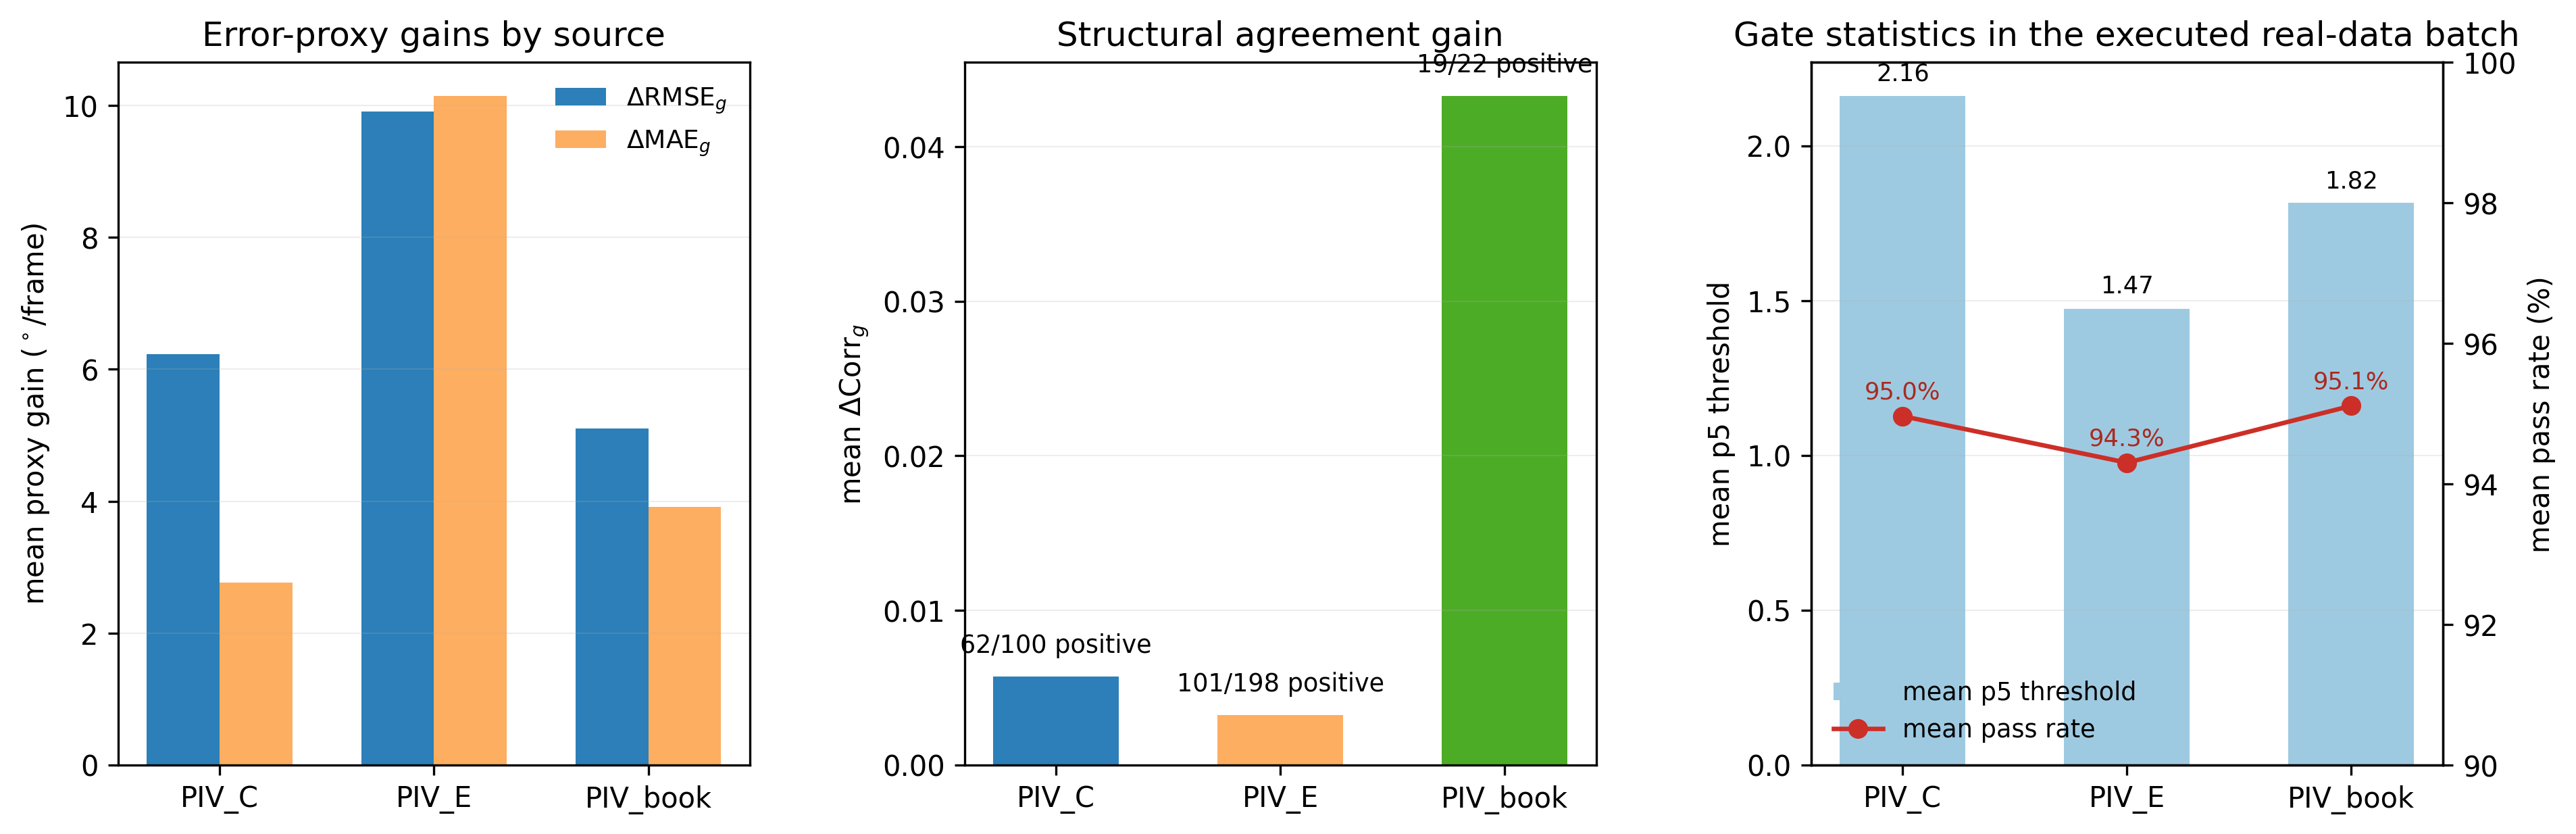
\includegraphics[width=\textwidth]{figures/appendix/figA11_real_source_summary.png}
  \caption{Source-wise real-data summary for the executed 320-pair batch.
  Left: mean proxy-error gains.
  Middle: mean structural-gain $\Delta \mathrm{Corr}_g$ with the number of positive pairs annotated above each bar.
  Right: pair-wise adaptive p5 threshold together with the retained pass rate.
  The figure complements the main-text real-data discussion by showing how the proxy improvements distribute across the three source pools.}
  \label{fig:app_real_sources}
\end{figure}

\begin{figure}[!t]
  \centering
  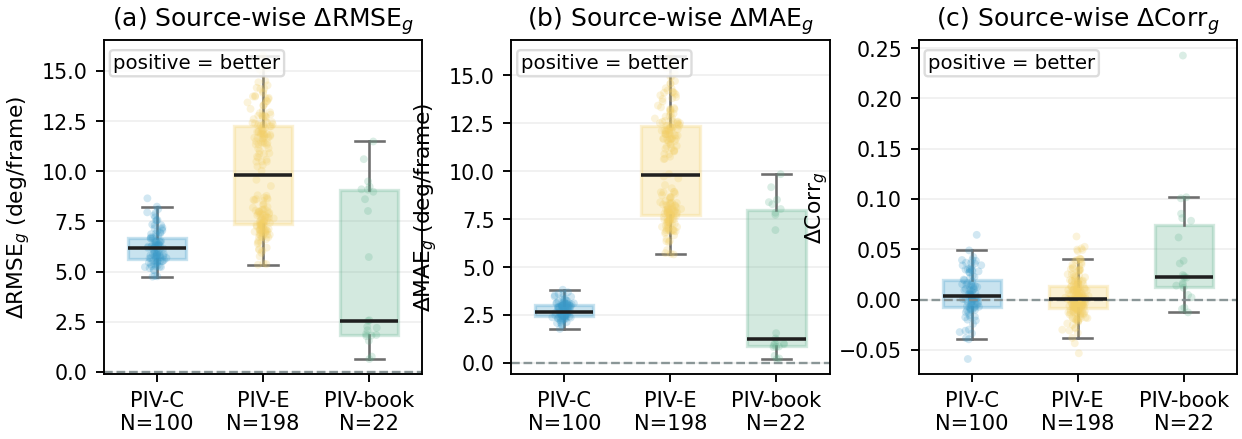
\includegraphics[width=\textwidth]{figures/appendix/figA16_real_proxy_distributions.png}
  \caption{Source-wise distributions of the real-data proxy gains across all 320 evaluated pairs.
  The three panels report $\Delta \mathrm{RMSE}_g$, $\Delta \mathrm{MAE}_g$, and $\Delta \mathrm{Corr}_g$ under the unified adaptive-$p_5$ protocol.
  These distributions were removed from the main-text representative-case figure to keep the real-case visualization compact.}
  \label{fig:app_real_proxy_distributions}
\end{figure}

\subsection{Representative Additional Real-Data Cases}

Fig.~\ref{fig:app_real_cases} reports one representative example from each executed
source pool.
The three cases act as source-level visual diagnostics that connect the batch statistics
to actual vorticity maps.
The chosen labels are PIV\_C `c099', PIV\_E `E\_camera\_3\_frame\_00050\_00051',
and PIV\_book `cam2\_5001', all of which lie in the stronger half of the corresponding
source-wise proxy-gain distribution while still showing clear interpretable structure.

\begin{figure}[!t]
  \centering
  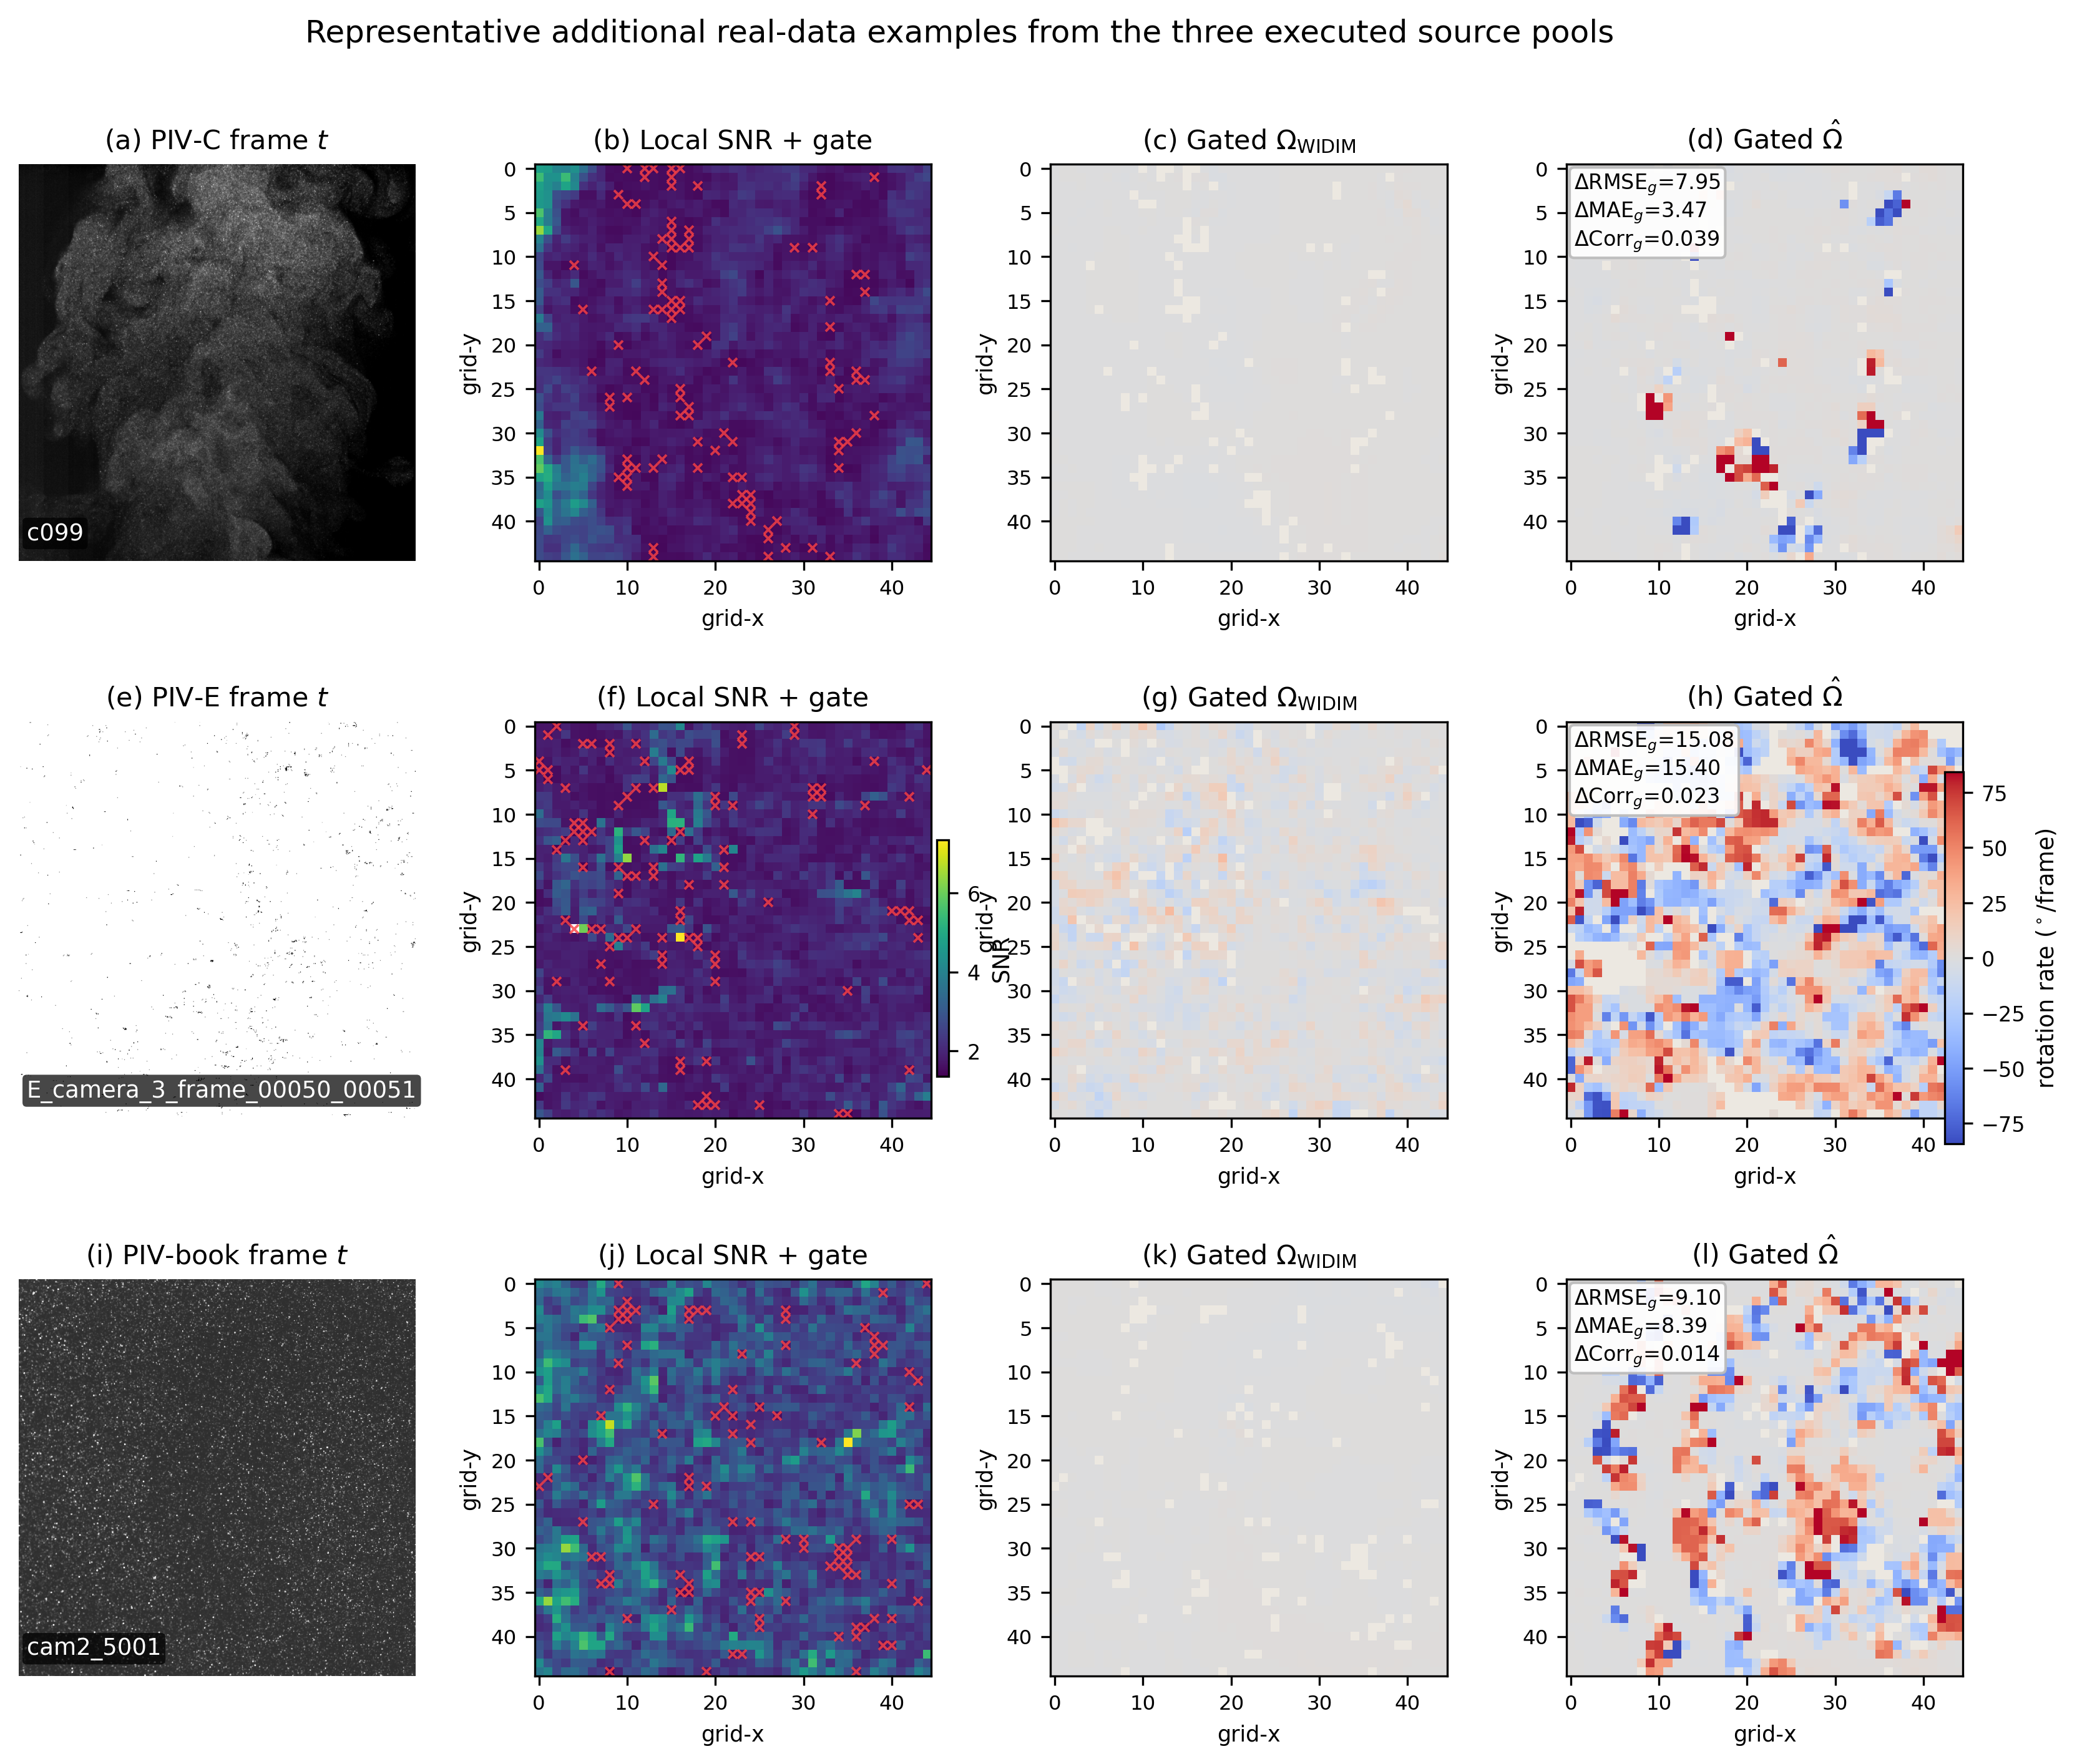
\includegraphics[width=\textwidth]{figures/appendix/figA12_real_source_cases.png}
  \caption{Additional representative real-data cases from the three executed source pools.
  Each row shows one source-specific example under the final protocol:
  the input frame, the local SNR map with rejected windows marked,
  the gated WIDIM-gradient reference map, and the final gated proposed map.
  The source-wise proxy gains reported in Table~\ref{tab:app_real_sources} are accompanied by
  visually interpretable flow structures rather than isolated numerical improvements.}
  \label{fig:app_real_cases}
\end{figure}

Among these three rows, the PIV\_book case `cam2\_5001' is the clearest
structural example:
the proposed field recovers a coherent vortex-ring-like pattern that is largely absent
from the WIDIM-gradient map.
For this reason, the main text uses `cam2\_5001' as the representative real-data figure.

Fig.~\ref{fig:app_real_boundary} adds a deliberately weaker case from PIV\_E.
Here the gain remains positive in the error-based proxies, but the visual difference
is much more modest.
This boundary example supports the discussion in the main paper that real-data gains
do not always appear as a dramatic new vortical structure;
in some scenes they appear primarily as tail suppression and local stabilization.

\begin{figure}[!t]
  \centering
  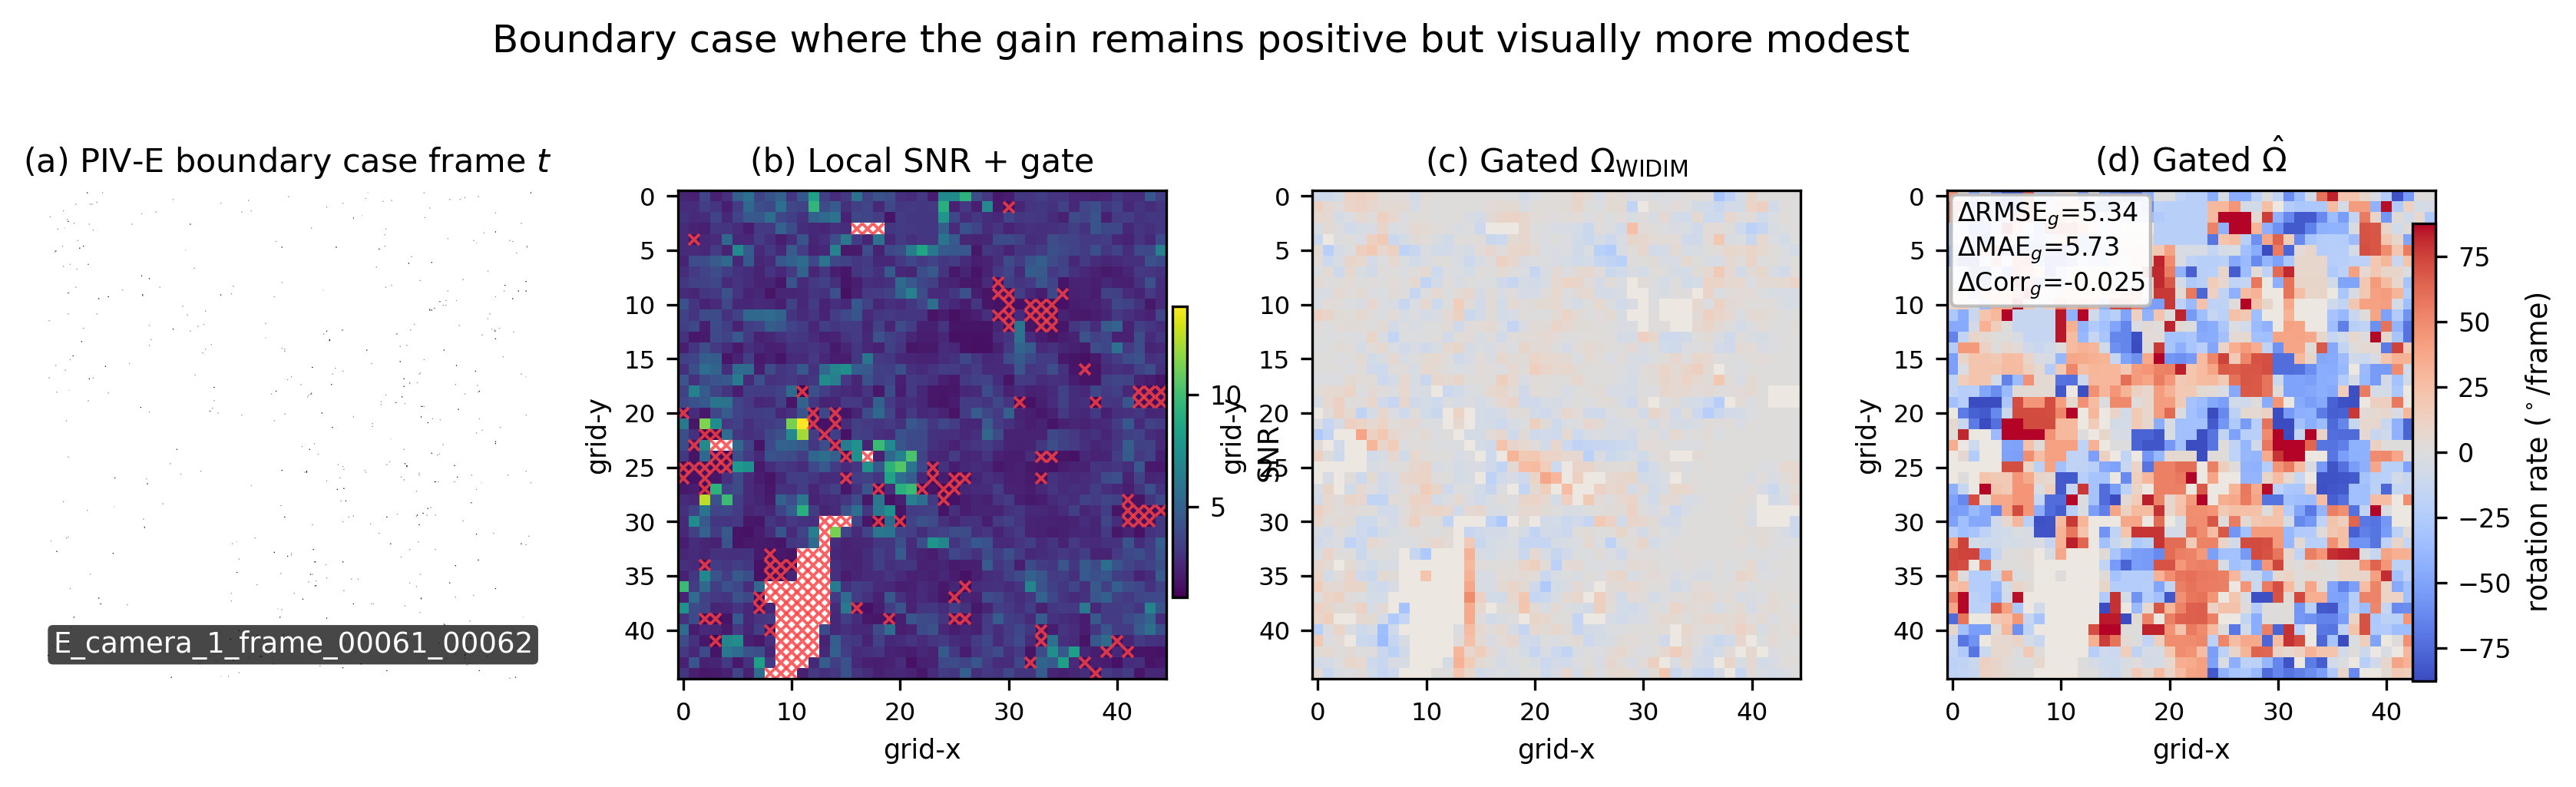
\includegraphics[width=\textwidth]{figures/appendix/figA13_real_boundary_case.png}
  \caption{Boundary real-data example with more modest visual gain.
  This PIV\_E case still shows positive proxy improvement under the final protocol,
  but the resulting difference is less dramatic than in `cam2\_5001'.
  The figure is included to show that the method's real-data gain can also appear as
  local stabilization and outlier suppression rather than as a newly visible coherent ring.}
  \label{fig:app_real_boundary}
\end{figure}

\FloatBarrier
\section{Absolute Protocol-Evolution Results Across V0--V3}
\label{app:evolution}

The main text uses a relative-gain summary to explain why the final deployable protocol
settles on V3.
For completeness, Table~\ref{tab:app_v0v3} and Fig.~\ref{fig:app_v0v3} retain the
absolute synthetic-flow RMSE values behind that summary.
Each protocol version is compared against its matched WIDIM baseline under the same evaluation setting:
V0 uses the idealized fixed-window setting, V1 and V2 use no-gate practical variants,
and V3 uses the final spatially gated protocol.

\begin{table}[!t]
  \centering
  \caption{Absolute synthetic-flow RMSEs across the V0--V3 protocol evolution.
  Each cell reports Proposed / WIDIM in degree per frame, with the lower value highlighted in bold.}
  \label{tab:app_v0v3}
  \small
  \renewcommand{\arraystretch}{1.12}
  \setlength{\tabcolsep}{4pt}
  \resizebox{\textwidth}{!}{%
  \begin{tabular}{@{}lcccc@{}}
    \toprule
    Flow & V0 fixed-window & V1 affine prior & V2 track prior & V3 final protocol \\
    \midrule
    Rankine &
    \textbf{0.416} / 1.037 &
    2.894 / \textbf{1.125} &
    6.517 / \textbf{1.125} &
    \textbf{0.864} / 1.102 \\
    Lamb-Oseen &
    \textbf{1.935} / 2.426 &
    3.377 / \textbf{2.484} &
    5.228 / \textbf{2.484} &
    \textbf{2.240} / 2.576 \\
    Solid rotation &
    0.271 / \textbf{0.223} &
    5.019 / \textbf{0.289} &
    \textbf{0.149} / 0.289 &
    \textbf{0.128} / 0.716 \\
    Linear shear &
    0.913 / \textbf{0.899} &
    \textbf{0.472} / 0.899 &
    0.907 / \textbf{0.899} &
    0.904 / \textbf{0.897} \\
    \bottomrule
  \end{tabular}}
\end{table}

\begin{figure}[!t]
  \centering
  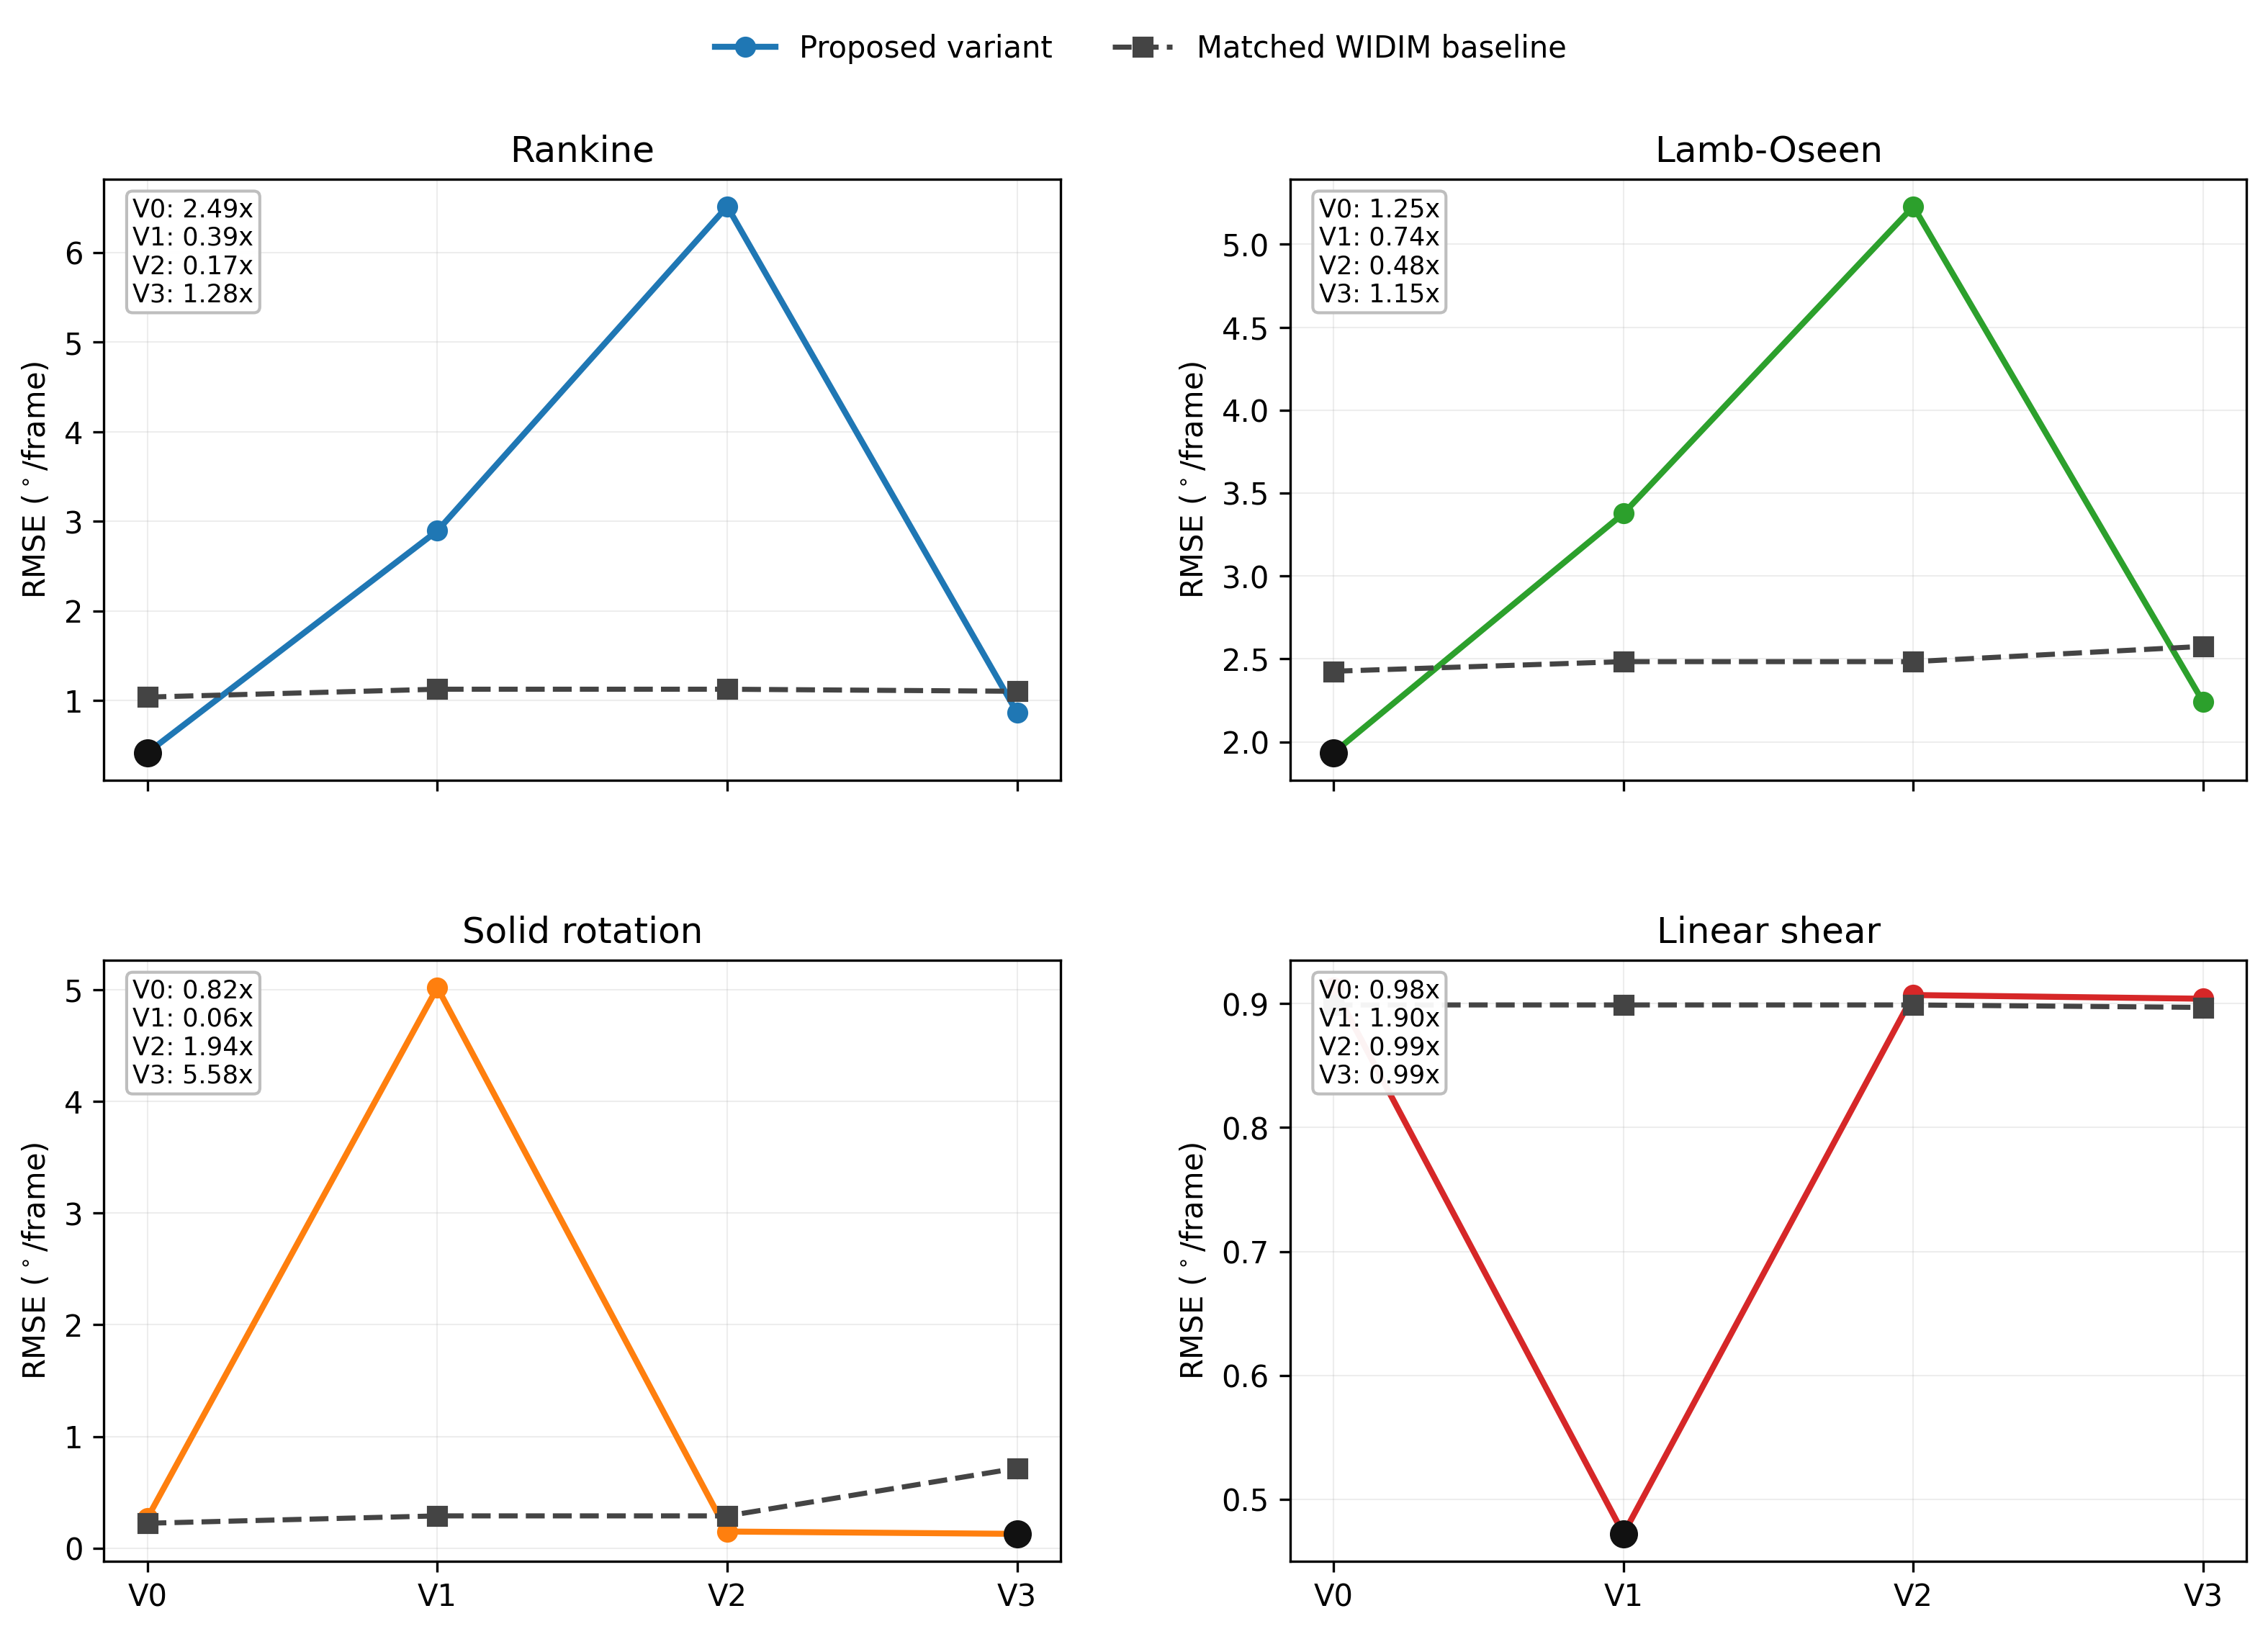
\includegraphics[width=\textwidth]{figures/appendix/figA14_protocol_evolution_absolute.png}
  \caption{Absolute protocol-evolution trajectories across the four synthetic flows.
  Solid lines plot the proposed-branch RMSE and dashed lines plot the matched WIDIM baseline.
  The figure makes the transition from the idealized V0 setting to the deployable V3 protocol explicit:
  V1 and V2 reveal the practical failure modes that motivate the final gated protocol,
  while V3 recovers the most stable cross-flow behavior.}
  \label{fig:app_v0v3}
\end{figure}

\FloatBarrier
\section{Implementation Details and Default Parameters}
\label{app:params}

For reproducibility, Table~\ref{tab:app_params} consolidates the default settings used
by the executable real-data pipeline.
The table is intentionally kept in the supplement rather than the main text because
these values support reimplementation and ablation reading, but are too detailed to
sit comfortably inside the primary scientific narrative.

\begin{table}[!t]
  \centering
  \caption{Default implementation parameters of the executed WIDIM(track)+NUFFT+Adaptive p5 pipeline.}
  \label{tab:app_params}
  \small
  \renewcommand{\arraystretch}{1.12}
  \setlength{\tabcolsep}{4pt}
  \begin{tabular}{@{}p{3.3cm}p{2.1cm}p{7.6cm}@{}}
    \toprule
    Component & Default value & Role in the executed pipeline \\
    \midrule
    Interrogation window size & $WS=64$ px & Common local window used by WIDIM tracking and the NUFFT branch. \\
    Real-data grid step & 10 px & Unified evaluation lattice for the real-data batch and the final reported proxy metrics. \\
    WIDIM iterations & 3 & Multi-pass displacement refinement before building the reference vorticity field. \\
    Search radius & 6 px & Translation search radius for tracked-window extraction. \\
    Search step & 1 px & Pixel stride used inside the local search. \\
    Translation prior & enabled & Only translational mismatch is removed before NUFFT; affine de-rotation is not used. \\
    Polar-spectrum inner cutoff & $r_{\min}=8$ & Removes the low-radius bins that are least informative for angular shift estimation. \\
    Spectral weighting & $r^2$ & Emphasizes higher-radius bins in the polar-spectrum correlation. \\
    Phase-only correlation & disabled & The final estimator uses standard correlation rather than POC in the deployed configuration. \\
    Pass-1 spatial gate & local MAD + weak-SNR/large-angle rejection & Rejects isolated spatial outliers before map refill. \\
    Weak-SNR angle rule & SNR $<2.2$ and $|\hat{\alpha}|>15^\circ$ & Explicitly removes the low-confidence large-angle spikes observed in practical windows. \\
    Pass-1 refill & trimmed mean, radius 1, 3 iterations & Restores rejected cells while suppressing single-point bursts. \\
    Pass-2 sign-island test & enabled & Detects isolated sign-opposite residual spikes after the first refill. \\
    Pass-2 refill & trimmed mean, radius 1, 2 iterations & Final local repair after the sign-opposite rejection pass. \\
    Adaptive gate & pair-wise p5 percentile & Keeps the tail-rejection policy fixed across all real-data pairs. \\
    Reported real-data metrics & $\Delta \mathrm{RMSE}_g$, $\Delta \mathrm{MAE}_g$, $\Delta \mathrm{Corr}_g$ & All three are computed on the same gated mask after the final post-process. \\
    \bottomrule
  \end{tabular}
\end{table}

\FloatBarrier
\section{Additional Runtime Diagnostics}
\label{app:runtime}

The main text intentionally keeps runtime discussion short so that the narrative stays
centered on the measurement path rather than software engineering details.
Fig.~\ref{fig:app_runtime} therefore places the extra timing diagnostics in the supplement.
Together with the source-wise mean execution times recorded in Table~\ref{tab:app_real_sources},
this figure shows that the current implementation is a research prototype:
the added cost of the direct-rotation branch is measurable but still moderate,
and the relative benefit of subpixel spectral fitting becomes more important as the window size grows.

\begin{figure}[!htbp]
  \centering
  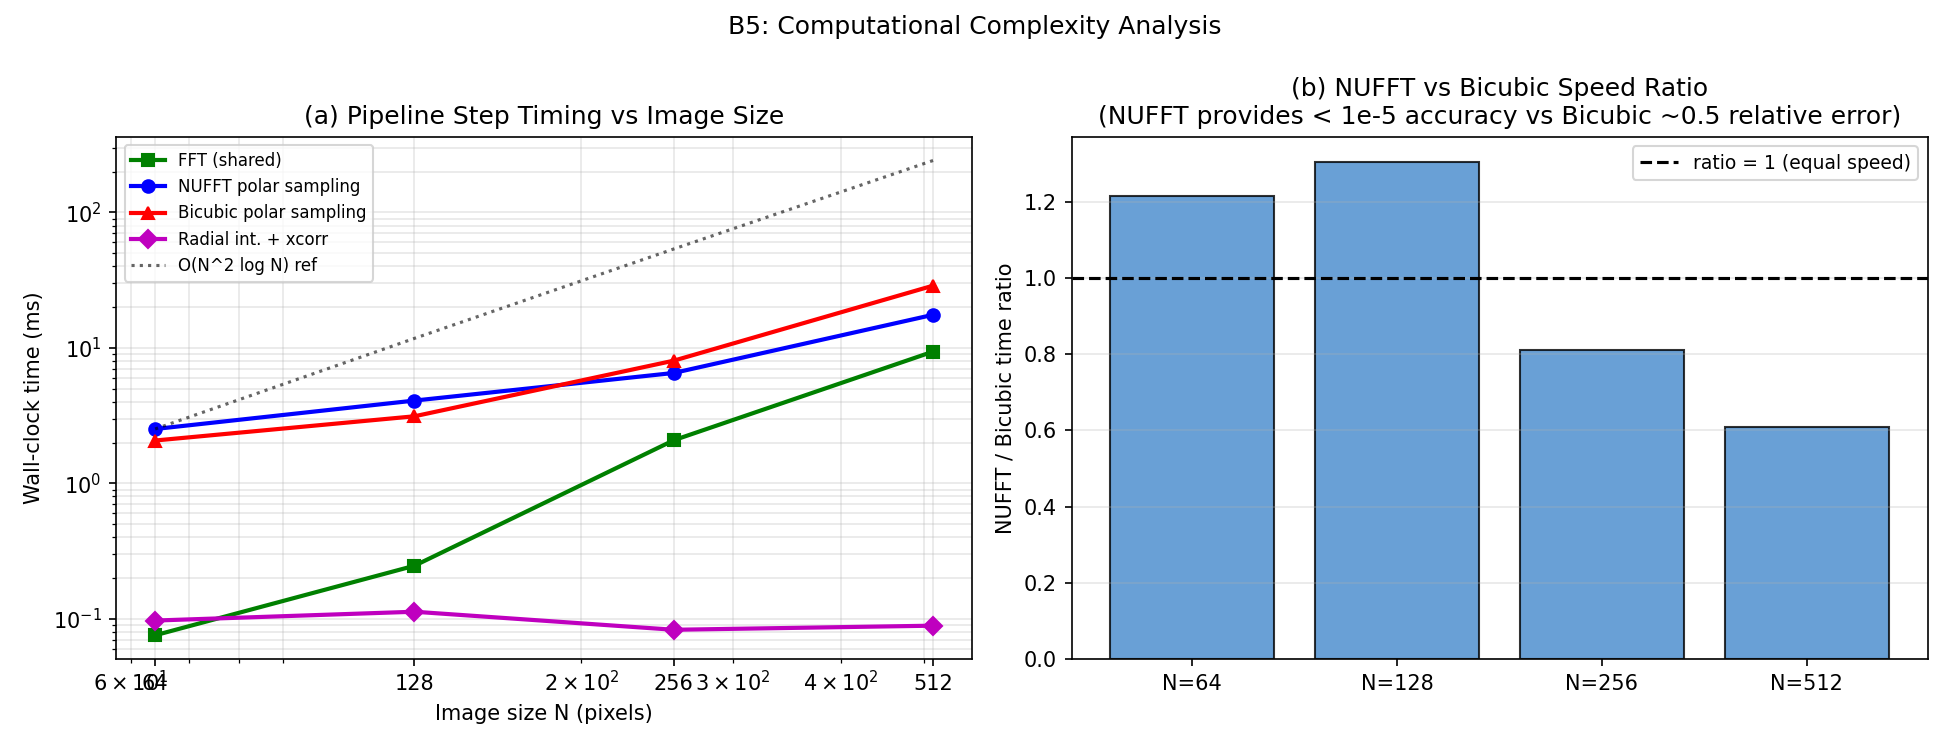
\includegraphics[width=\textwidth]{figures/appendix/figA15_runtime_complexity.png}
  \caption{Additional runtime and complexity diagnostics.
  Left: measured pipeline timing across representative image sizes and window settings.
  Right: relative cost of the NUFFT branch versus bicubic interpolation under the same experimental setup.
  This figure is included in the supplement because it supports implementation understanding but is not central to the paper's primary scientific claim.}
  \label{fig:app_runtime}
\end{figure}

\FloatBarrier
\bibliographystyle{IEEEtran}
\bibliography{refs}

\end{document}

